% options:
% thesis=B bachelor's thesis
% thesis=M master's thesis
% czech thesis in Czech language
% slovak thesis in Slovak language
% english thesis in English language
% hidelinks remove colour boxes around hyperlinks

\documentclass[thesis=M,czech]{FITthesis}[2012/06/26]

\usepackage[utf8]{inputenc} % LaTeX source encoded as UTF-8

\usepackage{graphicx} %graphics files inclusion
% \usepackage{amsmath} %advanced maths
% \usepackage{amssymb} %additional math symbols

\usepackage{dirtree} %directory tree visualisation
\usepackage{listings}

% % list of acronyms
% \usepackage[acronym,nonumberlist,toc,numberedsection=autolabel]{glossaries}
% \iflanguage{czech}{\renewcommand*{\acronymname}{Seznam pou{\v z}it{\' y}ch zkratek}}{}
% \makeglossaries

\newcommand{\tg}{\mathop{\mathrm{tg}}} %cesky tangens
\newcommand{\cotg}{\mathop{\mathrm{cotg}}} %cesky cotangens

% % % % % % % % % % % % % % % % % % % % % % % % % % % % % % 
% ODTUD DAL VSE ZMENTE
% % % % % % % % % % % % % % % % % % % % % % % % % % % % % % 

\department{Katedra počítačových systémů}
\title{Zpracování a analýza logů roamingového systému eduroam}
\authorGN{Václav} %(křestní) jméno (jména) autora
\authorFN{Mach} %příjmení autora
\authorWithDegrees{Bc. Václav Mach} %jméno autora včetně současných akademických titulů
\supervisor{Ing. Alexandru Mihnea Moucha, Ph.D.} 

\acknowledgements{
  % Doplňte, máte-li komu a za co děkovat. V~opačném případě úplně odstraňte tento příkaz.
  Chtěl bych poděkovat vedoucímu práce Ing. Alexandru M. Mouchovi za to, že se ujal vedení této práce.
  Také bych chtěl poděkovat Ing. Janu Tomáškovi za čas, který mi věnoval v~průběhu konzultací, 
  za všestranné rady a podporu při realizaci.
}
\abstractCS{
  
  % V~několika větách shrňte obsah a přínos této práce v~češtině. Po přečtení abstraktu by se čtenář měl mít čtenář dost informací pro rozhodnutí, zda chce Vaši práci číst.

  % Tato práce pojednává o~tvorbě systému pro analýzu a zpracování logů roamingového systému eduroam.
  Diplomová práce \emph{Zpracování a analýza logů roamingového systému eduroam}
  pojednává o~tvorbě systému \emph{etlog} pro analýzu a zpracování logů roamingového systému eduroam.
  Služba eduroam je celosvětový systém, který umožňuje uživatelům z~akademických institucí připojení k~Internetu
  především prostřednictvím Wi-Fi.
  Stav služby je možné sledovat pomocí log souborů, které jsou tvořeny na základě aktivity uživatelů.
  Na bázi těchto souborů byl vytvořen systém pro sledování stavu služby,
  tvorbu statistik, vyhledávání a~detekci anomálií.
  Vytvořený systém \emph{etlog} zpracovává aktivitu služby z~celé země a
  pomohl celkově zlepšit stav služby eduroam v~České republice.
}
\abstractEN{
  % Sem doplňte ekvivalent abstraktu Vaší práce v~angličtině.

  %This thesis is about creating a system for analysis and processing of logs of roaming system eduroam.
  The diploma thesis \emph{Analysis and Processing of Roaming Data from the Eduroam Networking System}
  deals with the creation of the system called \emph{etlog} for analysing and processing logs of eduroam networking system.
  The eduroam service is a worldwide system which allows users from academic institutions to connect to the Internet
  mostly by Wi-Fi.
  The state of the service can be observed by means of log files, which are created by users' activity.
  On the basis of these files, the system was created with the intention to monitor the service,
  produce statistics, search and detect anomalous states.
  The new system \emph{etlog} processes service activities from the whole country and it
  helped to improve the condition of eduroam service in the Czech Republic.
}
\placeForDeclarationOfAuthenticity{V~Praze}
\declarationOfAuthenticityOption{5} %volba Prohlášení (číslo 1-6)
\keywordsCS{
  % Nahraďte seznamem klíčových slov v češtině oddělených čárkou.
  eduroam, etlog, RADIUS, vyhledávání, zpracování, roaming, detekce,
  statistika, CESNET
}
\keywordsEN{
  % Nahraďte seznamem klíčových slov v angličtině oddělených čárkou.
  eduroam, etlog, RADIUS, searching, processing, roaming, detection,
  statistics, CESNET
}

\begin{document}

% \newacronym{CVUT}{{\v C}VUT}{{\v C}esk{\' e} vysok{\' e} u{\v c}en{\' i} technick{\' e} v Praze}
% \newacronym{FIT}{FIT}{Fakulta informa{\v c}n{\' i}ch technologi{\' i}}


% TODO - vlna

\begin{introduction}

  eduroam (zkratka pro education roaming)
  je celosvětová bezpečná roamingová služba vyvinutá pro mezinárodní výzkum a vzdělávací komunitu.
  eduroam vznikl v~Evropě a rychle se rozšířil ve výzkumné a vzdělávací komunitě. 
  V~současnosti je dostupný v~79 zemích po celém světě. \cite{eduroam_where}
  eduroam umožňuje studentům, výzkumníkům a zaměstnancům ze zapojených organizací získat připojení na Internet napříč areálem univerzity
  a při návštěvách dalších zapojených organizací jednoduše tím, že otevřou svůj přenosný počítač. \cite{what_is_eduroam}

  Služba eduroam poskytuje uživatelům způsob, jak se bezpečně připojit na Internet 
  v~libovolné ze zapojených organizací pomocí Wi-Fi.
  %\footnote{
  %  Wi-Fi (WiFi) je technologie, která umožňuje elektronickým zařízením připojení k bezdrátové síti pomocí rádiového signálu.
  %}. 
  \cite{what_is_eduroam}
  Služba je velmi kvalitně zabezpečena, uživatelské údaje jsou v~bezpečí, 
  protože eduroam je nesdílí s~navštěvovanou organizací, místo toho jsou přeposlány do domovské instituce uživatele, kde jsou ověřeny.

  Architektura eduroamu je postavena na následujícím principu:
  \begin{itemize}
    \item{Autentizace uživatele je vykonána na domovském IdP (Identity Provider, poskytovatel identity)
      s~použitím specifických autentizačních metod.} 
    \item{Autorizační rozhodnutí o~přístupu k~síťovým zdrojům následně po řádné autentizaci 
    je vykonáno SP (Service Provider, poskytovatel služby), kterým je typicky přístupový bod Wi-Fi.}
  \end{itemize}
  Aby bylo možné dopravit uživatelský požadavek na autentizaci a stejně tak odpověď 
  od poskytovatele služby k~domovskému poskytovateli identity a zpět, byl vytvořen celosvětový systém hierarchie RADIUS\footnote{
    RADIUS je síťový protokol, který umožňuje centrální autentizaci, autorizaci a management uživatelů, 
    kteří se připojují a využívají síťové služby.
    Protokol RADIUS je definován v~RFC 2865.
  }
  serverů.
  %\footnote{
  %  Server je obecné označení pro počítač nebo počítačový program, který poskytuje nebo realizuje nějaké služby.
  %}.
  Typicky každý poskytovatel identity nasazuje vlastní RADIUS server, který je připojený k~lokální databázi
  %\footnote{
  %  Databáze je organizovaná kolekce dat.
  %}
  uživatelů.
  Tento RADIUS server je připojen k~RADIUS serveru federační úrovně, který je podle pořadí připojen k~infrastruktuře RADIUS serverů vyšší úrovně
  nebo se může připojovat k~RADIUS serverům dynamicky. \cite{geant1} 
  Server federační úrovně obvykle provozuje státně příslušná NREN\footnote{
    NREN (National Research and Education Network) je specializovaný poskytovatel Internetu a nadstavbových služeb, 
    který se zaměřuje na podporu výzkumných a vzdělávacích komunit dané země.
  }.
  Zjednodušená hierarchie je zobrazena na obrázku \ref{fig:eduroam_hierarchy}.

  Protože uživatelé zadávají svá uživatelská jména ve formátu \uv{uživatel@realm}, 
  kde realm je část doménového jména poskytovatele identity, často používaná ve formě instituce.tld (tld - Top Level Domain, Doména nejvyššího řádu),
  mohou RADIUS servery tuto informaci využít ke směrování požadavku k~příslušnému následujícímu RADIUS serveru, 
  dokud požadavek nedosáhne RADIUS serveru poskytovatele identity. \cite{geant1}

  \begin{figure}
    \centering
      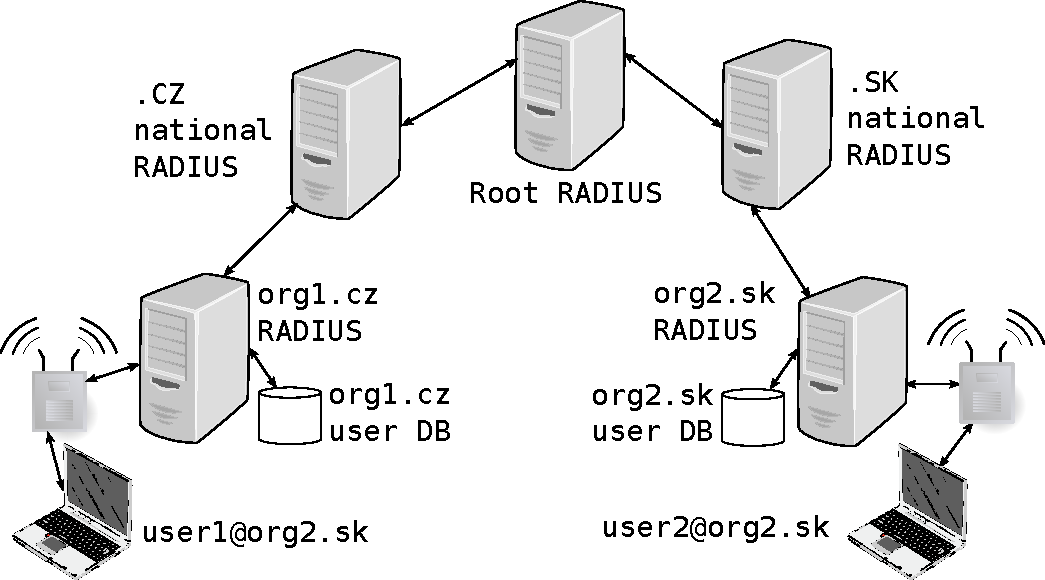
\includegraphics[scale=0.75]{eduroam-hierarchy.pdf}
    \caption[Hierarchie služby eduroam]{Zjednodušená hierarchie RADIUS serverů služby eduroam \cite{eduroam_caletka_pdf}}
    \label{fig:eduroam_hierarchy}
  \end{figure}

  Službu eduroam pro Českou republiku zajišťuje sdružení CESNET. 
  Z~výše popsané hierarchie vyplývá, že pokud je uživatel mimo svou domácí instituci,
  autentizační informace procházejí skrz hierarchii RADIUS serverů. 
  V~kontextu českého prostředí to znamená, že komunikace prochází skrze národní RADIUS server.
  Z~procházející komunikace je národní RADIUS server schopen vytvářet
  logy (záznamy) o~aktivitě uživatelů.

  Z~logů, které národní RADIUS server díky procesu popsanému v~předchozím odstavci získává,
  je možné zjistit mnoho různých informací o~fungování služby, o~jednotlivých organizacích a uživatelích.
  Pro zlepšování a kontinuální sledování kvality této služby bylo třeba vyvinout systém, 
  který zajistí potřebná data a bude informovat správce služby o~jejím stavu.

  %Navzdory pravidlům českého jazyka jsou 
  V~textu práce jsou občas na začátku věty malá písmena, když věta začíná názvem, který začíná malým písmenem.
  V~práci také používám některé anglické názvy, 
  které jsou v~daném kontextu běžně používány v~angličtině.

\end{introduction}

\chapter{Cíl práce}

  Cílem této práce je navržení a implementace systému pro zpracování a analýzu roamingových logů
  z~národního RADIUS serveru za účelem sledování kvality služby, trendů, 
  identifikace podezřelých událostí a chyb při ověřování uživatelů. 
  Tento systém by měl následně pomoci uživatelům služby, správcům jednotlivých institucí
  při řešení problému s~sledování stavu služby.
  V~neposlední řadě i sdružení CESNET, které národní RADIUS server spravuje.

  Pro uživatele by měl systém přinést lepší možnosti řešení problémů, které se potenciálně můžou vyskytnout.
  Pro správce služby by měl tento systém přispět možností sledování veškerých událostí týkajících se jejich instituce.
  Správci služby v~jednotlivých institucích by zároveň měli získat lepší přehled o~tom, 
  jak je služba využívána domovskými uživateli a kterým uživatelům cizích institucí je služba poskytována.
  Systém by měl současně vylepšit možnosti řešení uživatelských problémů tím, 
  že logy budou přímo přístupné správcům služby všech zapojených institucí.

  Před zahájením práce nad tímto tématem neexistoval žádný systém, který by byl schopen všechny zmíněné metriky sledovat a analyzovat.
  CESNET provozuje několik systémů, které sledují některé z~metrik služby, ale neprovozuje žádný komplexní systém.
  Kromě sledování metrik služby by mělo být výrazným přínosem reportování neobvyklých událostí.
  Mezi takové události by mohly patřit například nefunkčnost služby v~konkrétní lokalitě
  nebo nadměrný počet neúspěšných pokusů o~přihlášení.

  Navržený a implementovaný systém by měl mít obecné rozhraní, 
  aby bylo možné ho používat k~získání libovolných dat definovaných uživatelem nebo správcem.
  Rozhraní systému by mělo také umožnit strojové zpracování dostupných dat
  pro případné další analýzy nebo jiné účely.

\chapter{Analýza a návrh}

  Při práci na analýze a návrhu systému jsem spolupracoval se sdružením CESNET,
  které bylo zadavatelem tvorby systému.
  Tvorbu návrhu systému jsem konzultoval téměř výhradně s~Ing. Janem Tomáškem, a to z~několika důvodů:
  \begin{itemize}
    \item{Je správcem národního RADIUS serveru.}
    \item{Byl schopen zodpovědět všechny mé dotazy o~fungování služby.}
    \item{Měl konkrétní představu o~rozhraní systému a datech, která měl systém poskytovat.}
  \end{itemize}
  V~následujících částech textu budou často zaměňována slova systém a aplikace,
  obě slova představují realizovaný systém.

\section{Analýza}
 
  Ve fázi analýzy bylo třeba detailně porozumět procesu fungování autentizace
  uživatele v~hierarchii RADIUS serverů a roli národního RADIUS serveru, kde jsou logy generovány.

  \subsection{Fungování eduroamu}
    
    Služba eduroam je založena na protokolech IEEE 802.1X\footnote{
      IEEE 802.1X je protokol, který umožňuje zabezpečení přístupu do počítačové sítě.
      Protokol 802.1X je definován v~RFC 3579 a 3580.
    }
    a EAP\footnote{
     EAP (Extensible Authentication Protocol) je autentizační kostra často používaná v~bezdrátových sítích.
     Protokol EAP je definován v~RFC 3748.
    }.
    Hierarchie RADIUS serverů, které zajišťují AAA\footnote{
      Protokol AAA (Authentication, Authorization and Accounting) je rámec definující kontrolu přístupu, 
      zajišťování politik a auditování pro počítačové systémy.
      Protokol AAA je definován v~RFC 3539.
    }, může k~vzájemné výměně zpráv používat buď protokol RadSec\footnote{
      RadSec je protokol pro transport zpráv protokolu RADIUS pomocí TCP a TLS.
      Protokol RadSec je definován v~RFC 6614.
    }nebo protokol RADIUS.

  \subsubsection{IEEE 802.1X}
    Protokol IEEE 802.1X je běžně využívaný standard pro autentizaci uživatelů při přístupu k~síťovým službám. 
    Obrázek \ref{fig:8021x} popisuje schéma fungování protokolu.
    Fungování protokolu lze popsat následovně:
    \begin{itemize}
      \item{uživatel je připojen k~síti, veškerý jeho provoz je blokován nejbližším síťovým prvkem,}
      \item{autentikátor pošle uživatelskému zařízení výzvu k~autentizaci,}
      \item{klientské zařízení musí obsahovat nástroj supplicant, který naváže výměnu zpráv s~autentikátorem, 
        kde využije zadanou uživatelskou identitu,}
      \item{autentikátor předává klientské zprávy protokolem RADIUS nebo Diameter\footnote{
        Diameter je síťový protokol pro autentizaci, autorizaci a účtování.
        Protokol Diameter je definován v~RFC 3588 a 6733.
      } na autentizační server,}
      \item{v~případě, že uživatel je pomocí autentizačního serveru úspěšně ověřen, je uživateli povolen přístup do sítě bez omezení.}
    \end{itemize}

    Schéma sítě využívající protokol 802.1X je na obrázku \ref{fig:8021x_net}.
    Společně s~federací (hierarchií RADIUS serverů) eduroam umožňuje tento přístup
    ověřovaní lokálních uživatelů lokálně, tedy v~případě výpadku federace nedojde k~lokálnímu výpadku služby.
    Ostatní uživatelé jsou směrování pomocí realmu v~uživatelském jménu k~domovským autentizačním serverům.
    \cite{eduroam_caletka_pdf}

    \begin{figure}
      \centering
        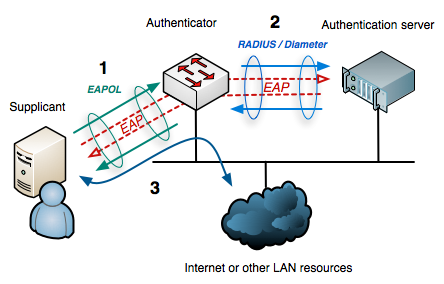
\includegraphics[scale=0.65]{8021x_net.png}
      \caption[Schéma sítě používající protokol IEEE 802.1X]{Schéma sítě používající protokol IEEE 802.1X \cite{eduroam_caletka_pdf}}
      \label{fig:8021x_net}
    \end{figure}

    \begin{figure}
      \centering
        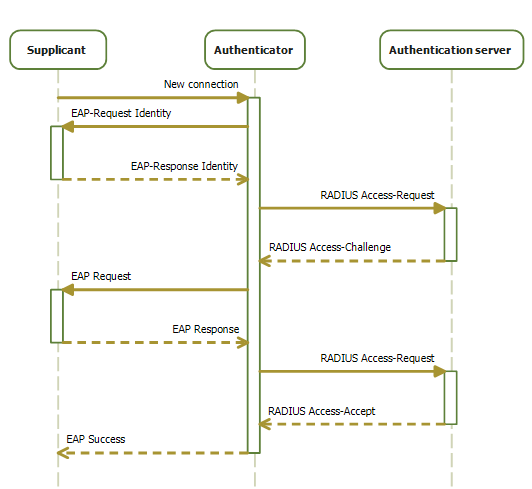
\includegraphics[scale=0.85]{8021x.png}
      \caption[Schéma fungování protokolu IEEE 802.1X]{Schéma fungování protokolu IEEE 802.1X \cite{8021x}}
      \label{fig:8021x}
    \end{figure}


  \subsubsection{EAP}
    
    Protokol EAP byl původně určen jako autentizační rozšíření pro protokol PPP\footnote{
      PPP (Point-to-Point Protocol) je protokol linkové vrstvy používaný pro přímé
      spojení dvou síťových uzlů.
      Protokol PPP je definován v~RFC 1661.
    }.
    Protokol PPP podporoval EAP od doby vzniku EAP jako alternativu k~CHAP\footnote{
      CHAP (Challenge-Handshake Authentication Protocol) slouží k~autentizaci
      uživatele nebo síťového zařízení.
      Protokol CHAP je definován v~RFC 1994.
    }a PAP\footnote{
      PAP (Password Authentication Protocol) je autentizační protokol, který využívá hesla.
      Protokol PAP je definován v~RFC 1334.
    }, které byly postupně začleněny do EAP.
    EAP je pouze autentizační kostra a nespecifikuje žádné konkrétní metody.
    Protokoly používající konkrétní metody jsou obvykle spojeny s~názvem metody.
    Často používané protokoly jsou například: EAP-TLS, EAP-TTLS, EAP-PEAP.
    
    Protokol EAP sám slouží pouze jako transportní médium pro ostatní protokoly
    a definuje pouze formáty zpráv\cite{rfc3748}.
    Konkrétní protokoly zapouzdřené pomocí EAP definují jakým způsobem 
    bude probíhat vlastní autentizace.
    V~českém prostředí se obvykle používá protokol EAP-PEAP,
    ale lze se setkat například i s~protokolem EAP-TLS.

    V~případě použití protokolu EAP-PEAP jsou uvnitř
    protokolu EAP zapouzdřena TLS data.
    Protokol TLS vytváří zabezpečený tunel mezi klientským
    zařízením a domovským RADIUS serverem.
    Data TLS tunelu, která jsou přenášena v~paketech EAP-Message, jsou šifrována.
    Obsah dat TLS tunelu je čitelný pouze pro klientské zařízení a domovský RADIUS server.
    Obrázek \ref{fig:eap_peap} detailně popisuje celý proces fungování protokolu EAP-PEAP.
    
    \begin{figure}
      \centering
        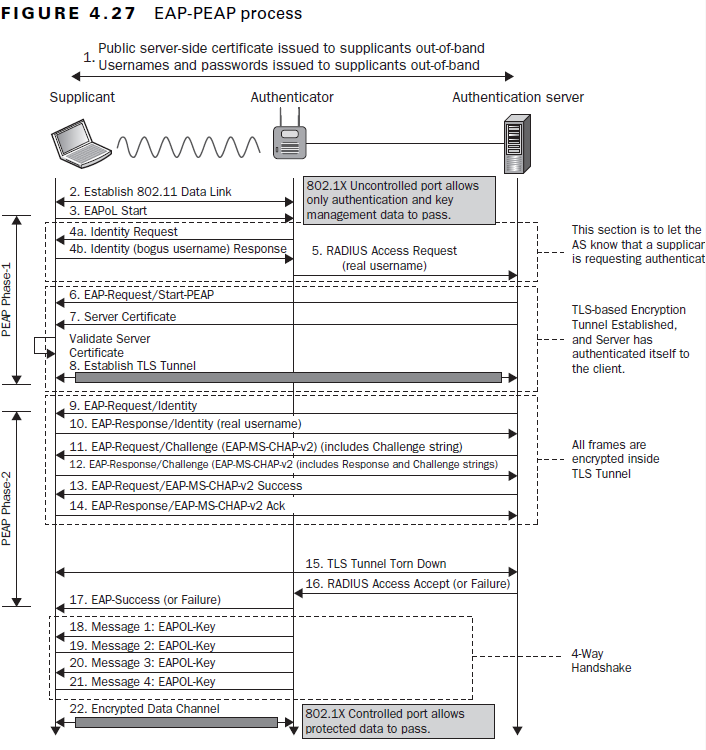
\includegraphics[scale=0.7]{eap-peap-20.png}
      \caption[Schéma fungování protokolu EAP-PEAP]{Schéma fungování protokolu EAP-PEAP \cite{eap_peap}}
      \label{fig:eap_peap}
    \end{figure}

    Z~obrázku je patrné, že pro udělení přístupu klientskému zařízení musí 
    být vyměněno mnoho zpráv.
    Každá vyměňovaná zpráva je zpracována národním RADIUS serverem
    a zaznamenána v~podobě části úplného log souboru (podrobněji je popsáno dále).
    Jedním z~podstatných důvodů práce s~redukovanými log soubory byl právě fakt, že
    úplné logy obsahují velké množství informací.

    Ostatní data protokolu RADIUS, která jsou součástí paketů,
    jsou čitelná pro všechny RADIUS servery, skrze které autentizační informace procházejí.
    Díky tomu je možné, aby byl vůbec požadavek směrován k~domovskému RADIUS serveru uživatele.
    Pro směrování požadavku je využita vnější identita, jejíž hodnota je v~uvedena v~atributu User-Name.
   
    Zprávy protokolu RADIUS jsou přenášeny nešifrovaně mezi 
    nejbližším síťovým prvkem (obvykle jde o~přístupový bod) a odpovědným RADIUS serverem.
    Pomocí sdíleného tajemství jsou šifrovány pouze atributy User-Password
    a Message-Authenticator. 
    Atribut User-Password se běžně při používání služby eduroam vůbec
    nevyskytuje, využívá s~pouze při autentizaci protokolem PAP.
    Atribut Message-Authenticator slouží k~zajištění integrity RADIUS paketu.
    %Uživatelské heslo je šifrováno pomocí sdíleného tajemství a je přenášeno
    %v~atributu User-Password.
    %Sdílené tajemství je taktéž využito v~atributu Message-Authenticator
    %pro zajištění integrity zprávy.
    Log soubory, které vznikají na základě uživatelské aktivity,
    jsou výsledkem zaznamenávání nešifrovaných částí procházejících RADIUS paketů.
    % pozorování nešifrovaných částí procházejících Access-Accept paketů.

  \subsubsection{RADIUS}
   
    Protokol RADIUS slouží k~předávání zpráv mezi RADIUS servery v~hierarchické struktuře služby.
    Protokol RADIUS používá pro výměnu zpráv protokol UDP\footnote{
      UDP (User Datagram Protocol) je jeden z~protokolů používaných v~Internetu.
      Protokol UDP je definován v~RFC 768.
    }.
    Použití protokolu UDP může být problematické z~důvodu fragmentace zpráv
    při přenosu přes různé síťové linky.
    Problémy může rovněž způsobit MTU\footnote{
      MTU (Maximum transmission unit) je označení pro maximální velikost IP datagramu, 
      který je možné konkrétním síťovým rozhraním odeslat.
    }
    společně s~větším objemem přenášených dat. \cite{eduroam_tutorial}
    Obrázek \ref{fig:eduroam_radius} ukazuje roli protokolu RADIUS v~eduroamu.

    \begin{figure}
      \centering
        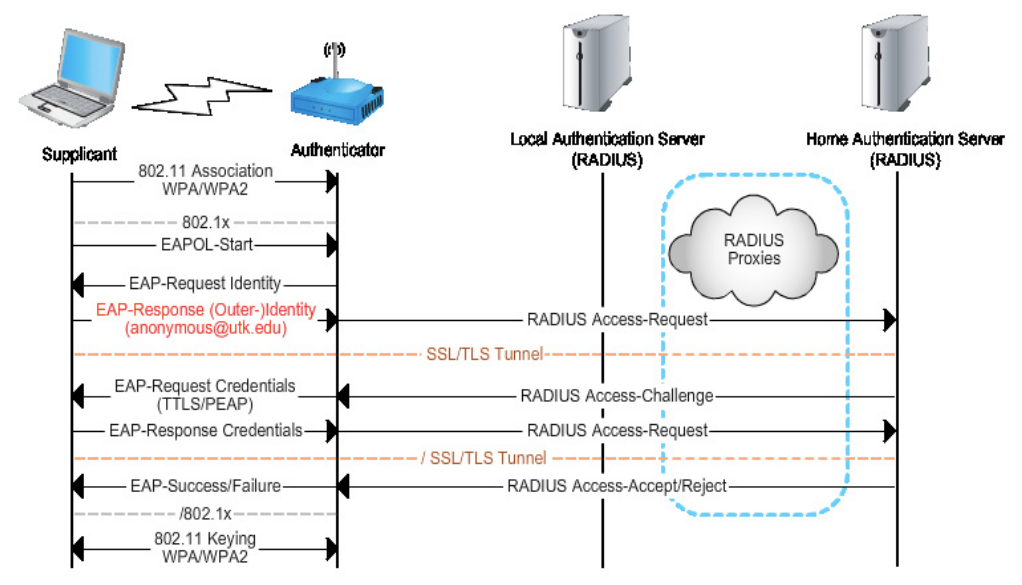
\includegraphics[scale=0.5]{eduroam_radius.png}
      \caption[Fungování protokolu RADIUS v~eduroamu]{Fungování protokolu RADIUS v~eduroamu \cite{eduroam_tutorial}}
      \label{fig:eduroam_radius}
    \end{figure}

  \subsubsection{RadSec}
    RADIUS k~přenosu paketů používá protokol UDP.
    %\footnote{
    %  UDP (User Datagram Protocol) je jeden z protokolů používaných v Internetu.
    %} 
    %protokol. 
    Protokol kromě uživatelského hesla nešifruje žádná data. 
    Protokol RadSec se snaží řešit jak problém ochrany přenášených dat před odposlechem a modifikací, 
    tak také spolehlivost přenosového kanálu. 
    Data jsou přenášena po TCP\footnote{
      TCP (Transmission Control Protocol) je jedním z~hlavních protokolů používaných v~Internetu.
      Protokol TCP je definován v~RFC 793.
    }
    a jsou šifrována pomocí TLS\footnote{
      TLS (Transport Layer Security) je kryptografický protokol, který zajišťuje zabezpečenou komunikaci v~počítačové síti.
      Protokol TLS je definován v~RFC 5246.
    }. 
    Protokol je specifikován v~RFC\footnote{
      RFC (Request for Comments) je označení dokumentů, které popisují zejména Internetové protokoly.
    }
    6613, specifikace vznikla rozvinutím Specifikace RadSec od společnosti OSC.\cite{eduroam_radsec}

  \subsection{Současný stav}

    Před vznikem navrženého systému byla situace následující.
    Logy byly generovány ve dvou formách.
    Úplná forma log souboru je tvořena laděním (debugging) obsahu příchozích EAP paketů\footnote{
      Paket je formátovaná jednotka dat přenášená v~počítačové síti.
    }, 
    je tedy značně obsáhlá.
    Detailní popis struktury úplné formy logů je popsán v~podsekci \ref{full_logs}.
    Redukovaná forma log souboru je zapisována ve formátu F-Ticks, více o~struktuře
    je popsáno v~podsekci \ref{reduced_logs}.
    
    Log soubory měly být primárně zdrojem informací o~stavu služby.
    Stav služby v~tomto kontextu představuje potenciální vyskytující se problémy,
    míru využívání, stav v~různých oblastech a další ukazatele.
    Při problému s~připojením do sítě u~konkrétního uživatele 
    bylo třeba lokalizovat zdroj problému.
    To pro správce služby znamenalo potřebu vyhledávání v~log souborech.
    Více o~samotném vyhledávání je popsáno v~podsekci \ref{searching}.

    Jedním z~důvodů potřeby tvorby systému pro analýzu byla taktéž skutečnost, 
    že množství informací zapisovaných do log souborů bylo značné a infrastruktura,
    kde je národní RADIUS server nasazen, byla již na hranici svých možností z~hlediska
    vstupně výstupních operací.
    Úplné logy nabývají velikosti přibližně 4 GB za hodinu, velikost redukovaného logu za
    jeden den je přibližně 100 MB.
    Protože uživatelů a zařízení používajících službu eduroam stále přibývá, 
    bylo třeba zohlednit i tuto skutečnost.

  \subsubsection{Úplné logy}
  \label{full_logs}

    Úplný log je tvořen čtyřmi hlavními typy záznamů.
    První dva typy zpráv jsou zprávy mezi autentikátorem a autentizačním serverem následně po tom, co supplicant poskytne uživatelskou identitu.
    Access-Request představuje žádost klienta a Access-Challenge reprezentuje odpověď serveru. 
    Jeden konkrétní záznam může vypadat například takto:

    \begin{verbatim}
Mon Oct 6 11:28:26 2014: DEBUG: Packet dump:
*** Received from 147.228.52.13 port 1814 ....
Code:
Access-Request
Identifier: 25
Authentic: m<199><200><240><166>zf<212>)<194><173>><178>4<254>|
Attributes:
User-Name = "user@cesnet.cz"
Chargeable-User-Identity = ""
Location-Capable = CIVIC_LOCATION
Calling-Station-Id = "ab-cd-ef-12-34-56"
Called-Station-Id = "00-13-5f-f8-b8-90:eduroam"
NAS-Port = 13
cisco-avpair = "audit-session-id=93e4cf04000302d1543260ba"
NAS-IP-Address = 147.228.207.4
NAS-Identifier = "ic-5508-wlc"
Airespace-WLAN-Id = 1
Service-Type = Framed-User
Framed-MTU = 1300
NAS-Port-Type = Wireless-IEEE-802-11
Tunnel-Type = 0:VLAN
Tunnel-Medium-Type = 0:802
Tunnel-Private-Group-ID = 128
EAP-Message = <2><1><0><20><1>user@cesnet.cz
Message-Authenticator = <176>Zj<231>F7<211>x<170>|<27><210>)p<244>S
Proxy-State = 193
    \end{verbatim}

    Uživatelské jméno (zde user@cesnet.cz) je přenášeno v~atributu User-Name.
    MAC adresa\footnote{
       MAC (Media Access Control, řízení přístupu k~médiu) adresa elektronického zařízení je unikátní identifikátor přiřazený síťovému rozhraní
      pro komunikaci na linkové vrstvě.
    } 
    uživatelského zařízení je obsažena v~atributu Calling-Station-Id (zde ab-cd-ef-12-34-56).
    Na základě poskytnutých údajů je uživateli udělen či odepřen přístup k~síti.
    Těmto stavům odpovídají typy zpráv Access-Accept a Access-Reject.
    Odpovídající Access-Accept k~ukázkovému záznamu výše je následující:
    
    \begin{verbatim}
Mon Oct 6 11:28:26 2014: DEBUG: Packet dump:
*** Sending to 147.228.52.13 port 1814 ....
Code:
Access-Accept
Identifier: 11
Authentic: 2<239>’<30>a<128><155><182><220><240><233><22><231><197>tt
Attributes:
User-Name = "user@cesnet.cz"
MS-MPPE-Send-Key = Yh^<184>H(nI<250><24><27><220><145><210>
"<140><218>f<145><178>P<21>$<249><172><2><153>kZ2<153>b
MS-MPPE-Recv-Key = <149><149><215><187><139>}<135><205>*<204>
<133><134><136>6<183><27><129>Q36<154>P#<<18><217>H<215><138><189>y<236>
EAP-Message = <3><13><0><4>
Message-Authenticator = <206><174>g<220><170><13><223><240>
<229>><230><14><128><206><252><130>
User-Name = "user@cesnet.cz"
Proxy-State = 205
    \end{verbatim}

    Z~těchto záznamů je patrné, že jsou velmi detailní a tudíž vhodné pro podrobnou analýzu. 
    Protože jsou však záznamy velmi detailní, zabírají taktéž velké množství místa.
    Pro účely základní analýzy postačují redukované logy.
    Nicméně, většina vyhledávání bohužel vyžaduje podrobnosti, které redukované logy neobsahují, 
    a proto je nutné vyhledávat v~úplných log souborech.

    Úplné logy jsou neocenitelné při řešení problémů s~autentizací a problémů v~infrastruktuře služby.
    Pozdější vylepšení infrastruktury, kde je národní RADIUS server nasazen,
    umožnilo sběr úplných logů bez výrazných problémů.
    Taktéž bylo upuštěno od vypisování obsahu paketů EAP-Message,
    protože jejich obsah neměl žádný význam při řešení problémů.
    Zadavatel definoval, že systém má být založen na redukovaných log souborech,
    úplné log soubory sloužily pouze k~hlubšímu pochopení této problematiky.

  \subsubsection{Redukované logy}
  \label{reduced_logs}

    Redukovaný záznam odpovídající dvěma uvedeným plným záznamům v~podkapitole \ref{full_logs} je následující:

    \begin{verbatim}
Oct 6 11:28:26 radius1mng2 fticks[11756]:
F-TICKS/eduroam/1.0#REALM=cesnet.cz#VISCOUNTRY=CZ
#VISINST=zcu.cz#CSI=ab-cd-ef-12-34-56#RESULT=OK
    \end{verbatim}

    Záznamy jsou zapisovány ve formátu F-Ticks. Nejedná se o~standardizovaný formát,
    ale pouze o~návrh, který je však ve federaci hojně využíván. \cite{monitor_eduroam}
    Návrh na standardizaci je publikován na webových
    %\footnote{
    %  Web (World Wide Web, WWW) je informační prostor, kde lze přistupovat k dokumentům a jiným webovým zdrojům.
    %}
    stránkách IETF\footnote{
      IETF (The Internet Engineering Task Force) je organizace, která tvoří a propaguje Internetové standardy.
    }.
    Dokument je dostupný na adrese 
    \href{https://tools.ietf.org/html/draft-johansson-fticks-00}{https://tools.ietf.org/html/draft-johansson-fticks-00}.
    Ze záhlaví dokumentu je zřejmé, že formát je vhodný jako zdroj pro analýzy:
    \uv{This document describes a log format for distributed identity
    federations that can be used as a tool for meetering and statistics
    gathering.}\cite{fticks_draft}

    Návrh definuje formát zpráv následovně dle ABNF\footnote{
      ABNF (Augmented Backus--Naur Form) je metajazyk využívaný pro zápis bezkontextových gramatik.
      Specifikace ABNF je definována v~RFC 4234.
    }:
    \begin{verbatim}
fticks = "F-TICKS/" federation-identifier "/" version attribute-list
label = ( ALPHA / DIGIT / '_' / '-' / ':' / '.' / ',' / ';')
federation-identifier = label
version = label
attribute-list = 1*("#" attribute "=" value ) "#"
value = label
attribute = ( ALPHA / DIGIT )
    \end{verbatim}

    Dále jsou definovány obecné atributy: REALM, VISCOUNTRY, VISINST, CSI, RESULT, RP, AP, TS, AM, PN.
    Definice atributů použitých v~ukázce výše je dle dokumentu následující:
    \begin{itemize}
      \item{REALM -- Sděluje AAA-oblast (například RADIUS) autentizační události}
      \item{VISCOUNTRY -- ISO\footnote{
        ISO (International Organization for Standardization, Mezinárodní organizace pro normalizaci) je světovou
        federací národních normalizačních organizací.
      }
      kód země entity, která vygenerovala zprávu}
      \item{VISINST -- Atribut není v~dokumentu specifikován}
      \item{CSI -- ID
      %\footnote{
      %  ID (Identifier) je jméno, které identifikuje unikátní objekt.
      %}
        volající stanice (Calling Station ID) subjektu spojeného s~autentizační událostí}
      \item{RESULT -- Výsledek autentizace buď 'OK' nebo 'FAIL'}
    \end{itemize}

    Ačkoliv dokument nedefinuje atribut VISINST, z~názvu atributu bylo možné odhadnout, 
    že reprezentuje jméno navštívené instituce. 
    Z~dostupných záznamů bylo zřejmé, že se jedná o~doménové jméno.
    Zadavatel rovněž předpokládal, že do budoucna bude formát rozšířen o~další z~obecných atributů.

  \subsubsection{Vyhledávání}
  \label{searching}
    
    % Vyhledávání znamenalo, že se objevil nějaký problém koncového uživatele.
    % Problém nejčastěji představoval uživatele, kterému se nedařilo službu použít.
    % Mohlo se ale jednat i o~zcizené uživatelské zařízení, které potenciálně mohlo službu opět využívat.
    
    V~případě výskytu nějakého problému, například
    problémů s~autentizací nějakého konkrétního uživatele,
    a nebo snaze o~lokalizaci zcizených uživatelských zařízení, která potenciálně mohla
    službu opět využívat, musel správce národního RADIUS serveru provést vyhledávání.
    % Všechny tyto případy znamenaly, že správce služby musel provést vyhledávání v~log souborech.
    Většina vyhledávání se prováděla nad úplnými log soubory, 
    kde bylo možné vzhledem k~množství obsažených informací jednoznačně určit zdroj problému.

    Pro samotné vyhledávání byl použit skript, který je přiložen níže.
    \begin{verbatim}
#!/usr/bin/perl -w

use strict;
use Data::Dumper;

my $file = $ARGV[1];
my $search = $ARGV[0];

open(F, "lzcat $file |") or die "Failed to read: $!";

my $record;
my $found = 0;

while (my $line = <F>) {
  $record .= $line;

  unless ($found) {
    $found++ if ($line =~ m/$search/o);
  };

  if ($line =~ /^$/) {
    # konec zaznamu v log souboru
    print $record if $found;
    $found = 0;
    $record = '';
  };
};
    \end{verbatim}

    Protože přiložený skript vyhledává přímo v~ladícím výstupu národního RADIUS serveru,     
    poskytuje kompletní obsah paketů,
    které byly vyměňovány mezi supplicantem a domovským RADIUS serverem.
    To umožňuje dohledat zdroj problému na nejnižší možné úrovni.
    Takovéto vyhledávání tudíž vyžaduje, aby správce, který hledání provádí,
    velmi dobře znal proces fungování služby.
    Na základě těchto znalostí lze jednoduše nalézt zdroj problému.

    Použití skriptu je omezeno parametry, kterými může být libovolný
    řetězec, který se vyskytuje v~samotných paketech.
    V~praxi to znamená, že parametrem hledání může být uživatelské jméno
    nebo MAC adresa.
    Tyto možnosti vyhledávání jsou pro základní potřeby správce služby dostatečné,
    ale pro zkoumání pokročilých metrik služby už je nelze použít.

    Doba běhu skriptu je výrazně závislá na počtu souborů, ve kterých je vyhledáváno.
    Vyhledávání v~souborech pro celý jeden den trvá okolo 15 minut.
    Doba běhu je výrazně ovlivněna tím, že soubory jsou ukládány v~komprimované formě.
    Doba vyhledávání v~nekomprimovaných datech je poloviční v~porovnání s~komprimovanými.
    
    Důvodem pro ukládání dat v~komprimované podobě je jejich velikost.
    Pro uložení je použita komprese LZMA\footnote{
      LZMA (Lempel--Ziv--Markov chain Algorithm) je algoritmus pro bezeztrátovou kompresi.
    }.
    Kompresní poměr je v~případě těchto konkrétních dat zhruba 20násobný.
    Soubory jsou generovány v~intervalu hodin. 
    Velikost souborů se různí v~závislosti na denní době.
    Typické velikosti komprimovaných souborů se pohybují od 40 do 150 MB.

    Nově navržený systém etlog by měl poskytovat značně rozsáhlejší možnosti vyhledávání.
    Základní vyhledávání mělo umožňovat vyhledávání podle uživatelského jména,
    MAC adresy, výsledku autentizace, časového intervalu nebo libovolné kombinace těchto parametrů.
    Pokročilé možnosti vyhledávání měly poskytovat především informace
    o~roamingu uživatelů, analýze trendů využívání lokalit a další podstatná data.

  \subsection{Požadavky na systém}

    Požadavky na systém definoval zadavatel v~průběhu konzultací.
    Jedním z~hlavních požadavků byla dostupnost.
    Vytvořený systém měl být dostupný pro jakéhokoliv uživatele (a případně i správce)
    ze zapojené organizace.

    Tím mělo být jednoznačně zajištěno, že libovolný uživatel z~jakékoliv zapojené organizace
    bude mít přístup k~systému, a tak potenciálně i k~informacím o~vlastním používání služby.
    Pokud by se objevil problém s~funkčností služby, měl by uživatel možnost dohledat
    potřebné informace, a tak by potenciálně mohl vyřešit problém sám.
    Pokud by uživatelé nebyli schopni řešit své problémy sami skrze systém,
    mohla by pro ně problémy řešit uživatelská podpora služby, pro kterou
    měl být systém taktéž dostupný.

    Dalším z~hlavních požadavků bylo uložení veškerých relevantních dat
    a vyhledávání v~nich.
    Uložení dat samo o~sobě nebylo problémem, 
    problémem byl počet vstupně výstupních operací a velikost uchovávaných dat.
    Data byla ukládána do souborů, což je standardní struktura poskytovaná operačním systémem.
    
    Z~hlediska omezení počtu vstupně výstupních operací existují efektivnější
    metody uložení dat než jsou soubory.
    Zadavatel rozhodl, že bude postačovat uchovávání informací dostupných v~redukovaných log souborech.
    Velikost dat tedy nebyla zásadním omezením. 
    Hlavním omezením tohoto požadavku bylo efektivní uložení dat takovým způsobem,
    aby bylo možné nad daty provádět vyhledávání a všechny definované analýzy.

    Dostupné redukované logy obsahovaly veškeré záznamy o~používání služby.
    To znamenalo, že jakákoliv zapojená organizace, která neměla svou infrastrukturu
    vhodně nakonfigurovanou, mohla generovat záznamy, které neodpovídaly formátu F-Ticks.
    Systém by tak mohl obsahovat data, která by mohla znesnadnit zpracování dat nebo negativně ovlivnit
    výsledky dostupných analýz.
    Z~této skutečnosti vyplynul požadavek na filtrování dat, která bude systém obsahovat.

    Systém měl být schopen zobrazovat statistiky využívání služby.
    Konkrétní způsob realizace statistik nebyl definován.
    Ačkoliv se jedná o~obecný požadavek, jeho konkrétnější podoba
    může být například:

    \begin{itemize}
      \item{počet uživatelů, kteří službu využili v~konkrétní organizaci za definované časové období}
      \item{seznam organizací, které nejvíce poskytovaly službu v~definovaném časovém období}
      \item{počet neúspěšných přihlášení pro konkrétní organizaci v~definovaném časovém období} 
      \item{seznam uživatelů, kteří využívali nadměrné počty zařízení v~definovaném časovém období}
    \end{itemize}
    
    Jedním z~důležitých požadavků byly periodické notifikace o~stavu služby.
    Mohlo se jednat o~sledování neobvyklých událostí služby,
    například velkého počtu neúspěšných přihlášení konkrétního uživatele.
    Další možností byla notifikace vycházející ze sledování 
    stavu služby v~konkrétní oblasti. 
    Pokud by náhle došlo k~nárůstu neúspěšných přihlášení, 
    mohlo by to signalizovat problém s~fungováním služby.
    V~obou zmíněných případech měl být správce služby notifikován,
    aby mohl vzniklou situaci řešit.

    Dalším neméně důležitým požadavkem byla tvorba statistik za uplynulá časová období.
    Z~vytvořených statistik by následně bylo možné například odhadovat
    trendy vývoje v~různých lokalitách, 
    rozšiřovat pokrytí v~hojně využívaných lokalitách a podobně.

    Z~podstaty dat, která měl systém obsahovat bylo zřejmé,
    že by měl být přístup k~systému zabezpečen tak, aby nebyla data dostupná komukoliv.
    Zadavatel určil, že by aplikace měla umožňovat blíže nespecifikovanou formu autentizace, 
    která by umožňovala uživatelům všech zapojených organizací přístup.
    Autentizace měla umožňovat rozlišit uživatele a správce služby.

\section{Návrh}

  Na základě požadavků na systém vyplynulo, že nejvhodnějším řešením bude realizovat systém jako webovou aplikaci. 
  Web je v~současné době standardním informačním médiem, a tak je možné k~němu přistupovat z~téměř libovolných zařízení.
  Webová aplikace tudíž umožní přístupnost pro všechny uživatele zapojených institucí. 
  Návrh byl taktéž založen na faktu, že uživatele bude v~rámci aplikace možné autentizovat.
  Zároveň bude možné v~aplikaci rozlišit běžné uživatele a správce, a na základě toho poskytnout přístup k~požadovaným informacím.

  Vytvořit systém jiným způsobem než jako webovou aplikaci by znamenalo mnoho možných problémů.
  Jinou potenciální možností by bylo například zvolit nativní aplikaci nebo mobilní aplikaci.
  V~obou případech nastává problém s~nedostupností na druhé jmenované platformě. 
  Tedy mobilní aplikaci není možné spustit na osobním počítači a naopak.

  S~ohledem na tento problém by bylo vhodnější vytvořit systém jako nativní aplikaci.
  Toto rozhodnutí by však přineslo mnoho dalších problémů -- různé operační systémy,
  různé architektury počítačů a podobně.
  Kvůli těmto důvodům považuji webovou aplikaci za nejlepší možnou variantu pro vytvořený systém.

  Jedna z~hlavních výhod webové aplikace je, že uživatelé jsou odstíněni od výše popsaných problémů
  pomocí webového prohlížeče.
  Webový prohlížeč v~tomto kontextu hraje roli mezivrstvy, 
  která zajistí vše potřebné pro korektní fungování systému.
  Není třeba řešit různé operační systémy, různé architektury 
  nebo jiná specifika uživatelských zařízení.

  Aplikace musela být schopna uchovat velké množství dat (řádově miliony záznamů o~aktivitě uživatelů) 
  a být schopna v~nich rychle vyhledávat.
  Rychlost vyhledávání může být nahlížena z~několika pohledů.
  V~kontextu některých výpočtů může být doba několika hodin považována za rychlý výpočet,
  ale v~kontextu jiných výpočtů může být považována naopak za pomalý.
  Rychlost vyhledávání nebyla nijak explicitně definována, proto jsem pracoval s~předpokladem,
  který vycházel z~mých zkušeností s~webovými aplikace.
  Předpokladem bylo udržet maximální dobu vyhledávání v~jednotkách nebo maximálně desítkách sekund.
  Taktéž bylo nutné počítat s~řádově desítkami uživatelů současně využívajících aplikaci.
  
  Řešením obou těchto požadavků bylo použít v~aplikaci takový způsob uložení dat,
  který oba tyto hlavní požadavky splní.
  Existuje několik možností, jak zajistit tyto dva hlavní požadavky na data systému.
  Z~přípustných možností jsem zvolil použití databáze.
  Databáze jsou navrženy přesně tak, aby byly schopny uchovat velké množství dat a současně v~těchto datech rychle vyhledávat.
  Možnosti konkrétních databází se samozřejmě různí.
  
  Po výběru databáze jako prostředku pro skladování dat bylo třeba analyzovat data, která bude databáze uchovávat.
  Na základě struktury dat bylo možné zvolit typ databáze tak, aby co nejlépe vyhovoval daným požadavkům.
  Hlavní částí dat, která měla databáze uchovávat, byly samotné záznamy log souborů.
  Záznamy jsou tvořeny atributy a jejich hodnotami, lze tedy říci,
  že se jedná o~dvojice klíčů a hodnot.

  Na základě tohoto pozorování jsem se rozhodl analyzovat
  možnost takzvaných NoSQL databází.
  NoSQL databáze zajišťují datové úložiště i zpracování dat jiným způsobem než
  pomocí tabulek a vzájemných vztahů, které se používají v~relačních databázích.
  Protože NoSQL databáze nepoužívají vzájemné relace,
  může být databázové schéma velice jednoduché.
  NoSQL databáze poskytují vysokou propustnost a zároveň
  umožňují vertikální i horizontální škálování.
  Tento typ databází je často využíván ve webových aplikacích reálného času.\cite{nosql}

  Reprezentace dat v~NoSQL databázích je navržena tak,
  aby více odpovídala strukturám používaným
  v~objektově orientovaném programování, v~porovnání se strukturami relačních databází.
  Toto je důležité zejména v~aplikacích s~méně složitými datovými strukturami.
  NoSQL databáze obvykle využívají nějaké úložiště typu klíč-hodnota nebo document-store.\cite{nosql}

  Na základě těchto faktů jsem navrhl využít NoSQL databázi,
  volba konkrétní databáze byla stále nejasná.
  Po studiu několika zdrojů (\cite{nosql}, \cite{db_comparsion}, \cite{db_comparsion2})
  %Na základě několika zdrojů 
  jsem navrhl pro implementaci systému etlog použít MongoDB.

  MongoDB je NoSQL databáze s~úložištěm typu document-store a je implementována v~jazyce C++.
  Databáze používá k~ukládání záznamů formát BSON, který je tvořen seznamem dvojic klíčů a hodnot.
  %BSON je efektivní při ukládání záznamů i při vyhledávání při porovnání s~formátem JSON. \cite{db_comparsion2}
  Při porovnání formátů BSON a JSON\footnote{
    JSON (JavaScript Object Notation) je otevřený standardizovaný formát, který používá datové objekty složené z~klíčů a hodnot.
  }
  je při ukládání záznamů i při vyhledávání formát BSON efektivnější. \cite{db_comparsion2}

  Velikost dokumentů ve formátu BSON je omezena na 16 MB.
  Pro větší dokumenty používá MongoDB GridFS,
  což je způsob, jak rozdělit jeden velký dokument na několik částí.
  Několik významných společností včetně Evropské organizace pro jaderný výzkum
  používá MongoDB pro své projekty.\cite{nosql}
  Na základě těchto faktů jsem byl přesvědčen, že by tato konkrétní databáze
  měla být vhodnou součástí realizovaného systému.

  Návrhem jazyka, ve kterém měl být systém implementován, byl JavaScript.
  JavaScript je znám především jako jazyk pro skriptování na straně klienta,
  je však možné ho použít i pro skriptování na straně serveru.
  Pro tento účel jsem navrhl využít Node.js (někdy též pouze Node nebo node), což je multiplatformní javascriptové běhové
  prostředí pro vývoj vysoce škálovatelných webových aplikací.
  
  Node.js je zaměřen na jednoduchý vývoj škálovatelných síťových aplikací.
  Mezi hlavní rysy Node.js patří asynchronnost vstupně výstupních operací
  a jeho architektura založená na událostech.
  Výhoda použití tohoto jazyka může spočívat v~tom,
  že umožňuje vývojáři použít jeden jazyk pro skriptování na straně
  serveru i pro skriptování na straně klienta.\cite{nodejs}

  Přestože obě technologie existují krátkou dobu (méně než 10 let),
  je možné se s~nimi setkat v~mnohých významných projektech.
  Většina projektů využívá tyto technologie, protože
  aplikace, ve kterých jsou použity,
  pracují v~reálném čase a zpracovávají značné objemy dat.

  Kombinace Node.js a MongoDB by poskytovala výhodné možnosti pro tvorbu systému.
  MongoDB je schopno pracovat s~několika nativními datovými typy jazyka JavaScript.
  Jde především o~datový typ Date, který reprezentuje datum a čas.
  Tento typ byl z~podstaty ukládaných dat velmi důležitý. 
  Potenciální konverze, které by musely být prováděny před a po přístupu k~databázi
  v~případě výběru jiného jazyka, by mohly výrazně ovlivnit rychlost prováděných výpočtů.
  
  Další výhodou použití obou technologií zároveň bylo množství dostupných materiálů.
  Pro Node.js je dostupné nepřeberné množství modulů,
  které usnadňují použití a komunikaci s~MongoDB.
  Dostupné materiály taktéž zahrnují ukázky použití,
  dokumentaci a popis různých problémů.
  
  Společným použitím obou technologií by bylo možné horizontální i vertikální škálování.
  To znamená, že v~případě nedostatečného výkonu
  by mohly být navýšeny výpočetní prostředky serveru,
  kde by byl systém nasazen, 
  nebo by mohl být systém nasazen na několika různých serverech s~možností dodatečně zvýšit jejich počet.
  
  Volbu konkrétních součástí systému,
  například konkrétního webového nebo emailového serveru, jsem ponechal na proces realizace.
  V~této přípravné fázi práce nebylo podle mého názoru vhodné tyto komponenty
  stanovovat dopředu, protože prozatím nebylo zřejmé, 
  jakou konkrétní funkcionalitu budou v~systému realizovat a jak budou vzájemně propojeny.
  Systém měl být na základě návrhu realizován 
  jako webová aplikace pomocí Node.js jako aplikační kostry a pomocí databáze MongoDB.

  %Přestože systém sám neměl hrát v hierarchii RADIUS serverů žádnou roli,
  %bylo třeba navrhnout
  %Systém měl být v hierarchii služby zapojen takovým způsobem,
  %.. 

  %Obrázek ..
  %ukazuje návrh zapojení serveru v rámci hierarchie služby.

  % TODO - pridat obrazek hierarchie, ktery ukaze mne prideleny server

\chapter{Realizace}

  Projekt byl nazván etlog, což představuje zkratku pro eduroam traffic log analysis.
  Pro větší možnosti znovupoužitelnosti a rozšiřitelnosti je veškerá dokumentace 
  včetně zdrojových kódů a komentářů psána v~anglickém jazyce.
  Repozitář se zdrojovými kódy a dokumentací je dostupný na webové stránce \href{https://github.com/CESNET/etlog}{https://github.com/CESNET/etlog}.
  Vše je verzováno v~Gitu, což je distribuovaný systém pro správu verzí.
  Při realizaci jsem opět spolupracoval s~Ing. Janem Tomáškem, 
  protože měl konkrétní představy o~fungování a vzhledu celého systému včetně webového rozhraní.

  \section{Nastavení produkčního prostředí}

    Pro nasazení systému mi byl zřízen virtuální server.
    Bylo mu přiděleno doménové jméno
    %\footnote{
    %  Doménové jméno (Internetová doména) je řetězec, který jednoznačně identifikuje počítač nebo počítačovou síť, která je
    %  připojena do Internetu.
    %} 
    etlog.cesnet.cz. Server má přidělené 4 procesory a 16 GB operační paměti (paměti RAM\footnote{
      Paměť RAM (Random-access memory) je typ počítačového úložiště používaný k~ukládání často používaných instrukcí programů
      za účelem zvýšení celkové rychlosti systému. 
    }
    ).
    Jako operační systém serveru byl zvolen Debian\footnote{
      Debian je Linuxový operační systém.
    }
    ve verzi označené Jessie.
    Operační systém bylo třeba následně konfigurovat, 
    instalovat podpůrné softwarové balíčky a provádět dodatečnou údržbu.
    
    Diagram systému etlog zobrazující všechny podstatné části popsané v~této kapitole
    je na obrázku \ref{fig:etlog_diagram}.

    \begin{figure}
      \centering
        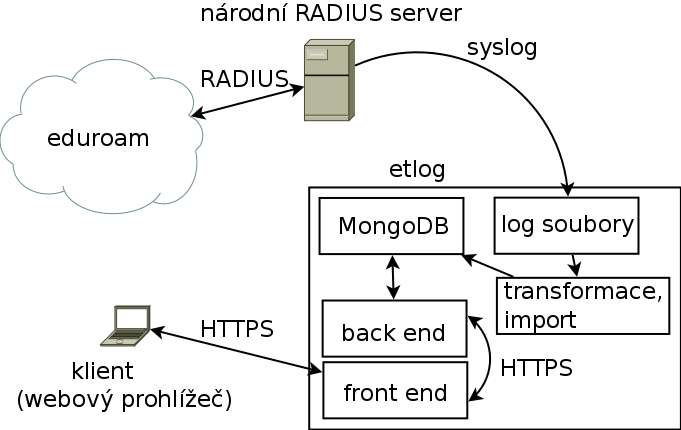
\includegraphics[scale=0.5]{etlog_diagram.png}
      \caption[Diagram systému etlog]{Diagram systému etlog}
      \label{fig:etlog_diagram}
    \end{figure}

    Pro potřeby aplikace jsem v~operačním systému vytvořil nového uživatele.
    Uživatel byl nazván etlog stejně jako celý projekt.
    Samostatný neprivilegovaný uživatel představoval několik výhod, které jsou rozebrány dále v~textu.
    Spuštění aplikace pod identitou neprivilegovaného uživatele však představovalo problém s~přístupností aplikace.
 
    \subsection{Síť}
    
      Neprivilegovaní uživatelé nemají možnost využívání síťových
      portů\footnote{
        V~kontextu protokolu IP je port koncový bod komunikace v~operačním systému.
      }
      s~číslem nižším než 1024.
      Porty 0 - 1023 mohou využívat pouze privilegovaní uživatelé.
      Protože aplikace měla být dostupná na standardních portech pro web,
      kterými jsou porty 80 a 443, bylo třeba tento problém vyřešit.
      Z~toho důvodu jsem se nejdříve zaměřil na dodatečnou konfiguraci sítě.

      Aby bylo možné do aplikace přistoupit pomocí přiděleného doménového jména,
      bylo třeba použít přístupné porty a na nich aplikaci spustit.
      Toto by znamenalo, že by aplikace již byla přístupná,
      uživatelé by se však stále nebyli schopni do aplikace dostat,
      museli by navíc znát čísla používaných portů.
      Bylo tedy nutné používané porty přesměrovat na standardní porty.
      Aplikace využívá porty 8080 a 8443.
     
      Aplikace je nastavena tak, že je přístupná pouze lokálně.
      Toto opatření je zavedeno jako jeden z~několika stupňů bezpečnosti.
      Pro propojení externí sítě s~interní jsem použil nástroj iptables-persistent,
      což je nadstavba iptables\footnote{
        iptables je program, který umožňuje administrátorům konfigurovat tabulky jádra Linuxového firewallu.        
      }.
      K~propojení interní a externí sítě jsem přidal i přesměrování používaných portů na standardní porty.
      Přesměrování je provedeno následujícím způsobem (pro názornost jsou příkazy uvedeny na více řádcích):

      \begin{verbatim}
iptables -t nat -A PREROUTING -i eth0 -p tcp \
  --dport 80  -j REDIRECT --to-port 8080
iptables -t nat -A PREROUTING -i eth0 -p tcp \
  --dport 443 -j REDIRECT --to-port 8443
iptables-save > /etc/iptables/rules.v4
ip6tables -t nat -A PREROUTING -i eth0 -p tcp \
  -d 2001:718:1:1f:50:56ff:feee:150/64 --dport 80 \
  -j REDIRECT --to-port 8080
ip6tables -t nat -A PREROUTING -i eth0 -p tcp \
  -d 2001:718:1:1f:50:56ff:feee:150/64 --dport 443 \
  -j REDIRECT --to-port 8443
ip6tables-save > /etc/iptables/rules.v6
      \end{verbatim}

      Nástroj iptables-persistent přidává iptables tu hlavní funkcionalitu, že pravidla,
      která jsou definována, jsou uložena a v~případě problému nebo údržby (například restartu serveru) opět načtena.
      Tím je tedy zajištěna perzistence pravidel.
      Pomocí tohoto nástroje jsem problém s~dostupností úspěšně vyřešil tak, aby byla aplikace dostupná obvyklým způsobem.
 
    \subsection{syslog}
    
      Dále bylo třeba vyřešit lokální přístupnost samotných F-Ticks log souborů pro aplikaci.
      Log soubory se generují přímo na národním RADIUS serveru.
      Řešením, které navrhl zadavatel, byl příjem záznamů pomocí protokolu syslog\footnote{
        Protokol syslog je standard pro zaznamenávání zpráv a je definován v~RFC 3164 a 5424.
      }.
      Pomocí konfigurace syslog démona\footnote{
        V~kontextu operačních systémů je démon počítačový program, který je spuštěn na pozadí.  
      }
      bylo možné definovat, že při zapisování záznamů
      lokálně na národním RADIUS serveru budou záznamy taktéž přeposílány
      na mně přidělený server.

      Na mnou používaném serveru následně stačilo instalovat
      softwarový balík syslog-ng a přidat následující dodatečnou konfiguraci:
      
      \begin{verbatim}
source net {
  tcp(
    port(1999)
    tls( ca_dir("/etc/ssl/certs")
    key-file("/home/etlog/etlog/cert/etlog.cesnet.cz.key.pem")
    cert-file("/home/etlog/etlog/cert/etlog.cesnet.cz.crt.pem"))
  );
};

destination fticks { 
  file("/home/etlog/logs/fticks/fticks-$YEAR-$MONTH-$DAY" 
  owner("etlog") group("etlog") perm(0600)); 
};

log { source(net); destination(fticks); };
      \end{verbatim}

      Generované log soubory byly ukládány do domovského adresáře
      uživatele etlog.
      Důvodem pro umístění v~domovském adresáři byla čitelnost pro neprivilegovaného uživatele a
      jednotné umístění všech log souborů souvisejících s~aplikací.

    \subsection{Emailový server}

      Další důležitou součástí aplikace byly reporty, které byly závislé na emailovém serveru.
      Jako emailový server byl zvolen Postfix.
      Při instalaci byl zvolen typ konfigurace \verb|Internet site|.
      Všechna ostatní nastavení byla ponechána beze změn.
      Server je omezen pouze na lokální poslech z~bezpečnostních důvodů.
      Žádné jiné restrikce nejsou definovány.

      Aplikace je s~emailovým serverem propojena pomocí modulu Nodemailer.
      Modul umožňuje definovat mnoho různých nastavení, která definují propojení
      aplikace s~emailovým serverem.
      Pro produkční nastavení jsem použil port 25. 
      Poslech emailového serveru je omezen pouze na lokální síť,
      protože v~rámci aplikace měl sloužit pouze pro odesílání emailů a nikoliv pro příjem.

      %Protože poslech emailového serveru byl omezen pouze na lokální síť,
      %nijak jsem neřešil šifrování spojení mezi emailovým serverem a aplikací.

    \subsection{Databáze}

      MongoDB je dokumentově orientovaná databáze.
      Pod pojmem dokumentově orientovaná databáze si lze představit
      záznamy, které jsou tvořeny vždy alespoň jedním klíčem a hodnotou.
      Tento formát je nazván JSON.
      %.
      MongoDB používá rozšířený JSON formát, kterým je BSON.
      %\footnote{
      % BSON (Binary JSON) je formát pro datovou výměnu používaný jako úložiště v databázi MongoDB.
      %}.
      Na nejvyšší úrovni je databáze (v~tomto kontextu databázový server) rozdělena do jednotlivých databází.
      Dále je databáze strukturována do kolekcí, které jsou obdobou tabulek SQL\footnote{
        SQL (Structured Query Language) je speciální programovací jazyk určený pro management dat uložených v~relačních databázích.
      }
      databází.
      Na nejnižší úrovni už se nacházejí samotné záznamy.

      V~repozitářích Debianu Jessie je dostupná pouze starší verze (2.4) instalačního balíčku.
      Na základě vylepšení dostupných v~aktuální verzi jsem se rozhodl ji instalovat.
      Instalovanou verzí byla verze 3.2, která oproti verzi 2.4 poskytovala mnoho různých vylepšení.
      V~aplikaci jsem pracoval především s~agregačním rozhraním, které bylo od doby dřívějších verzí značně vylepšeno.

      Pro instalaci bylo nutné přidat oficiální MongoDB repozitář do systémem
      používaných zdrojů pro instalaci softwarových balíků, a také importovat veřejný GPG\footnote{
        GPG (GNU Privacy Guard) je kryptografický software.
      }
      klíč MongoDB.
      Následně mohla být instalována nová verze MongoDB.

      Po instalaci jsem ověřil funkčnost databáze pomocí terminálového klienta \verb|mongo|.
      Po spuštění a připojení k~databázi bylo vypsáno následující varování:
      \begin{verbatim}
** WARNING: /sys/kernel/mm/transparent_hugepage/defrag is 'always.'
**        We suggest setting it to 'never'
      \end{verbatim}
      Dokumentace MongoDB o~této problematice říká: \uv{Transparent Huge Pages (THP) is a Linux memory management system that 
      reduces the overhead of Translation Lookaside Buffer (TLB) 
      lookups on machines with large amounts of memory by using larger memory pages.
      However, database workloads often perform poorly with THP, 
      because they tend to have sparse rather than contiguous memory access patterns. 
      You should disable THP on Linux machines to ensure best performance with MongoDB.}\cite{mongo_thp}
      Na základě těchto informací jsem se rozhodl databázi dodatečně konfigurovat.
      
      Zakázání THP by dle dokumentace mělo umožnit nejlepší výkonnost MongoDB.
      Dokumentace uvádí několik způsobů, jak THP zakázat.
      Vybral jsem zákaz pomocí takzvaného init skriptu, který je spuštěn vždy při startu operačního systému. 
      Skript zakáže THP pomocí zápisu do části souborového systému jádra operačního systému.
    
    \subsection{Zálohování}

      Další důležitou součástí nastavení produkčního prostředí bylo zálohování.
      Zálohování umožňuje navrátit obsah souborů a případně i databáze do dřívějšího stavu.
      Pomocí zálohování bylo možné jednoduchým způsobem přejít k~dřívějšímu stavu v~případě závažného problému.
      Pro zálohování byl zvolen nástroj duply, který je běžně používán sdružením CESNET.
      
      Konfigurace duply je velmi jednoduchá, přestože se jedná o~velmi propracovaný nástroj.
      Nástroj duply je pouze front endem pro duplicity,
      což je aplikace pro tvorbu šifrovaných inkrementálních záloh na vzdálená úložiště.\cite{duply}
      Konfigurace je tvořena především soubory conf a exclude.
      Konfigurační soubor conf definuje symetrický klíč a další možnosti šifrování,
      dále je definováno vzdálené úložiště a počet a stáří záloh.
      Konfigurační soubor exclude definuje, které adresáře mají být zálohovány a které ne.

      Pro zálohování bylo třeba dodat další součást konfigurace, kterou
      je jednoduchý skript, který je spuštěn před zahájením vlastní zálohy.
      Tento skript byl určen k~zálohování obsahu databáze.
      MongoDB poskytuje několik různých způsobů zálohování.
      Ze všech dostupných způsobů jsem vybral zálohování pomocí nástroje mongodump.
      Nástroj mongodump vytváří adresářovou strukturu, která obsahuje binární data databáze.
      
      Tento přístup má několik výhod.
      Vytvářená adresářová struktura se nijak nemění, pouze jsou při každém zálohování přepisována data.
      Díky tomu nejsou při následném zálohování data nijak duplikována.
      Přestože jsou obsahem souborů binární data, duply je schopno tvořit jejich inkrementální zálohy.
      Nevýhodou tohoto přístupu je větší objem potřebný k~uložení dat.

    \subsection{Periodické úkony}
      
      Systém potřebuje periodicky provádět různé úkony.
      Pro tento účel jsem využil cron\footnote{
        cron je časový plánovač úloh pro Unixové systémy.
      }, což je obvyklý způsob realizace periodických úkonů pro Unixové systémy.
      Prováděné úkony byly rozděleny podle toho, zda bylo nutné,
      aby je prováděl privilegovaný uživatel.

      Pro oba typy uživatelů jsem použil crontab\footnote{
        crontab je soubor, který obsahuje definice časů a příkazů, které mají být prováděny.
      }.
      crontab uživatele root provádí pouze jednu úlohu, kterou je zálohování.
      Kromě úkonů popsaných níže provádí aplikace i další, ty jsou detailně popsány v~sekci back endu \ref{backend}.
      crontab uživatele etlog provádí tyto úkony:

      \begin{center}
        \begin{tabular}{ | c | c | }
          \hline
            čas spuštění          & popis                                      \\ \hline
            každých 5 minut       & úloha pro import dat                       \\ \hline
            každý den v~01:00     & zpracování invalidních záznamů             \\ \hline
            každé pondělí v~06:00 & report o~invalidních záznamech             \\ \hline
            každé pondělí v~06:05 & archivace                                  \\ \hline
            každé pondělí v~06:10 & generování grafů o~počtech přihlášení      \\
          \hline
        \end{tabular}
      \end{center}

  \section{Zpracování log souborů}
    \label{logs_processing}

    \subsection{Transformace dat}

      Příchozí data byla postupně přidávána do souborů, pro každý den byl vytvářen vlastní soubor.
      Data bylo třeba transformovat z~formátu F-Ticks do formátu BSON, který používá MongoDB.
      Formát dat byl od doby analýzy změněn. Záznam v~novém formátu mohl vypadat následovně 
      (pro názornost uvedeno na více řádcích):

      \begin{verbatim}
Jan 1 08:00:00 195.113.187.36 fticks[151596]: 
F-TICKS/eduroam/1.0#REALM=cesnet.cz#VISCOUNTRY=CZ
#VISINST=1zcu.cz#CSI=ab-cd-ef-12-34-56#PN=user@cesnet.cz#RESULT=OK
      \end{verbatim}

      Změny ve formátu se týkají přidaného atributu PN a změny obsahu atributu VISINST.
      Atribut PN je v~návrhu formátu definován jako unikátní identifikátor subjektu, 
      kterého se týká autentizační událost.
      Zároveň je připojeno bezpečnostní doporučení, které říká, že
      atribut by měl být být maskován kryptografickou hashovací funkcí\footnote{
        Kryptografická hashovací funkce je s~funkce s~takovými vlastnostmi, které umožňují její použití pro zabezpečení informací.
      }
      před odesláním, aby nedocházelo k~úniku citlivých uživatelských informací.
      Protože je zabezpečen samotný přístup k~datům, není atribut nijak maskován.
      Jelikož je v~atributu uvedeno uživatelské jméno, jsou tím zároveň značně vylepšeny možnosti vyhledávání.
      Změna obsahu atributu VISINST představovala přidání znaku \verb|1| před vlastní obsah.
      Důvodem je použití hodnoty atributu Operator-Name, který je postupně do eduroamu zaváděn.\cite{rfc5580}

      Zadavatel do budoucna předpokládal ještě další rozšíření formátu.
      Jednalo se o~atribut RESULT, který měl být rozšířen o~další možnou hodnotu TIMEOUT.
      Před dokončením systému nebylo ještě rozšíření přidáno, 
      přesto by měl být systém schopen s~ním bez velkých problémů pracovat.

      Pro transformaci dat mezi formáty jsem vytvořil transformační skript\footnote{
        Skript je počítačový program napsaný ve skriptovacím jazyce.        
      }.
      Pro transformační jádro skriptu jsem zvolil jazyk AWK\footnote{
        AWK je programovací jazyk navržený na zpracování textu 
        a typicky používaný pro extrakci dat.
      }, zbylá část je psána v~Bashi\footnote{
        Bash je jeden z~Unixových shellů, který interpretuje příkazový řádek.
      }.
      Skript je bohatě komentován.
      Při samotné transformaci bylo třeba vyřešit dva hlavní problémy:
      \begin{itemize}
        \item{Jak určit aktuální rok?}
        \item{Jak číst pouze tu část dat, která ještě nebyla přečtena?}
      \end{itemize}

      Standardním vstupem počáteční implementace skriptu byla samotná data, která bylo třeba transformovat.
      Tento přístup se ukázal jako nevhodný, protože nebylo možné logické zapouzdření.
      Následující implementace pracovala pouze s~názvem log souboru, který měl být zpracován.
      Tento přístup se ukázal jako o~mnoho vhodnější. 
      Z~názvu souboru bylo možné jednoduše odvodit aktuální rok, 
      ověřovat, zda soubor existuje a provádět další podstatné operace.
      Název log souboru může mít například podobu \verb|fticks-2016-10-15|.

      Už při implementaci transformace dat bylo třeba brát v~potaz to,
      že transformační skript bude volán opakovaně v~pravidelných intervalech.
      Pokud by byl vstupní soubor při každém spuštění čten celý, docházelo by
      k~duplikování dat při importu do databáze.
      Z~toho důvodu bylo třeba zajistit, 
      aby každé následující spuštění skriptu pokračovalo ve čtení přesně v~místě,
      kde předchozí čtení skončilo.
      Pro tento účel jsem využil standardní nástroj logtail, který je navržen právě pro tento účel.

      Funkčnost služby eduroam je automaticky testována na jednotlivých institucích.
      Pro toto automatizované testování je vyhrazen rozsah MAC adres začínající znaky \verb|706f6c69|.
      Zbylá část adresy může být libovolná. 
      Protože se jedná o~umělá data, není žádoucí, aby byla analyzována.
      Z~toho důvodu transformační skript ignoruje všechny záznamy, 
      které obsahují zmíněný prefix MAC adresy používaný pro monitorovací účely.

      Obsah atributů samotných dat byl zadáván uživatelem, mohl být tudíž zcela libovolný.
      Analýza dat ukázala, že malé množství záznamů obsahuje různé netisknutelné znaky.
      Protože textová data byla transformována na řetězce, bylo třeba tyto 
      netisknutelné znaky nahradit.
      Každý netisknutelný znak je nahrazen řetězcem odpovídajícím jeho číselnému kódu v~ASCII\footnote{
        ASCII (American Standard Code for Information Interchange) je standard pro kódování znaků.
      }.
      Tedy například znak s~dekadickým kódem 8 je nahrazen řetězcem \verb|<8>|.

      Protože data obsahovala značný počet záznamů, které nesplňovaly požadavky pro jednotlivé atributy,
      bylo třeba tyto záznamy přeskakovat a ohlašovat.
      Hlášení o~chybných záznamech bylo směrováno na standardní chybový výstup.
      Obsahem hlášení je název souboru, ve kterém se vyskytla chyba, a číslo problematického řádku.
      
      Problém opět nastává při opakovaném spouštění transformačního skriptu.
      Při opětovném spuštění je na standardní vstup AWK předána pouze dosud nepřečtená část dat. 
      To znamená, že číslování řádek vůči vstupnímu log souboru je pouze relativní.
      Pro hlášení chyb je třeba absolutní číslování řádek, v~důsledku toho
      je třeba ukládat číslo poslední zpracované řádky a při dalším spuštění
      k~němu připočítat relativní číslo řádky. Tím je tento problém vyřešen.

      Transformační skript musel taktéž řešit různé formáty MAC adres,
      které mohou zapojené organizace poskytovat.
      Existující formáty MAC adres mohou vypadat následovně: 123456789abc, 12:34:56:78:9a:bc, 12-34-56-78-9a-bc, 1234.5678.9abc
      Adresy mohou taktéž obsahovat jak malá tak velká písmena.
      Všechny adresy jsou na výstupu normalizovány do jednotného formátu s~malými písmeny bez oddělovačů.

      Data jsou ze záznamů jednoduše extrahována -- atributy jsou vzájemně odděleny pomocí znaku \#.
      Hodnota je od jména atributu oddělena pomocí znaku =.
      Samotná extrakce dat je tedy snadná.
      Výstup může být například (pro názornost uvedeno na více řádcích):
      \begin{verbatim}
{ 
  timestamp : 
    { 
      "$date" : 1430956800000 
    }, 
  realm : "cesnet.cz", 
  viscountry : "CZ", 
  visinst : "zcu.cz", 
  csi : "abcdef123456", 
  pn : "user@cesnet.cz", 
  result : "OK" 
}
      \end{verbatim}

    \subsection{Import dat}
      Import dat bylo třeba provádět kontinuálně, stejně tak jako data přicházela.
      Importovaná data musela být samozřejmě v~nativním formátu databáze MongoDB -- 
      zde byl využit dříve implementovaný transformační skript.
      Pro import dat v~pravidelných intervalech jsem použil cron.
      Data jsou importována každých 5 minut.
      Vlastní úlohu pro import dat jsem napsal v~Bashi. 

      Problém nastává při zpracování posledního nezpracovaného intervalu dat (23:55-23:59)
      každého dne. Spuštění úlohy pro import dat každých 5 minut znamená, že
      úloha je spuštěna ve 23:55 a následně až v~00:00. 
      Druhé spuštění úlohy už ale probíhá v~následující den. Z~toho důvodu bylo
      nutné si ukládat datum při spuštění úlohy a při dalším spuštění ho porovnat s~aktuálním datem.
      V~případě, že se obě data lišila, došlo ke zpracování posledního intervalu předchozího dne.

      Vlastní import dat bylo možné řešit jednoduše pomocí programu mongoimport,
      který je součástí instalačního balíčku MongoDB a je určen právě pro import dat.
      Využil jsem přepínače programu mongoimport, 
      které umožňují specifikovat jméno kolekce i databáze.
      
      Potenciálním problémem bylo řešení duplicitních dat.
      Samotná databáze umožňuje zamezení existence duplicitních dat pomocí vytvoření unikátního indexu\footnote{
        Index je pomocná datová struktura umožňující rychlé vyhledávání.
      }.
      Program mongoimport taktéž nabízí přepínač -{}-upsertFields, pomocí kterého je možné definovat
      výčet polí, která mají být použita pro kontrolu, zda je každý jednotlivý vkládaný dokument unikátní.
      Při shodě všech definovaných polí není dokument do databáze importován.
      Značnou nevýhodou je nutnost prohledávání databáze při vkládání každého záznamu,
      z~čehož vyplývá, že použití přepínače velmi výrazně zpomalí import.
      Protože aktuální data nemohla být importována několikrát a vícenásobný import hrozil pouze u~starších dat,
      rozhodl jsem se tento problém ignorovat a zamezit mu precizním importováním starých dat.

      Import starších dat, která byla k~dispozici ještě před započetím implementace, bylo třeba řešit odděleně.
      Pro tato data jsem vytvořil samostatný skript. Stejně jako ostatní skripty je psán v~Bashi.
      Jako kostru jsem použil importní skript.
      Bylo třeba přidat funkcionalitu, která umožní zpracovat konkrétní log soubor. 
      To jsem realizoval pomocí parametru na příkazové řádce, který představuje datum log souboru, který má být zpracován.
      Dalším rozšířením bylo smazání podpůrných souborů transformace 
      pro zpracovávaný log soubor před jeho zpracováním, pokud existovaly.
      Nebylo třeba se zabývat problémem se zpracováním posledního intervalu ve dni, tuto část jsem tedy neřešil.

  \section{Struktura databáze}

    Databáze byla nazvána stejně jako samotná aplikace, tedy etlog.
    Databáze je strukturována do kolekcí, kolekce obsahují samotné dokumenty.
    Všechny dokumenty v~databázi implicitně obsahují klíč \verb|_id|,
    který slouží pro interní účely databáze.

    Vlastní transformované záznamy jsou ukládány do kolekce nazvané logs.
    Každý dokument v~této kolekci obsahuje klíče, které odpovídají všem atributům redukovaných logů.
    Všechny klíče kolekce kromě viscountry jsou indexovány pro efektivní vyhledávání.
    Indexování klíče viscountry nemělo pro prováděné analýzy žádný význam.

    Všechny kolekce, které jsou popsány níže a obsahují časovou známku události,
    mají hodnotu tohoto klíče vyplněnou uměle. 
    Umělá hodnota byla stanovena na začátek každého nového dne.
    Tato hodnota byl zvolena podle požadavků zadavatele, který určil, že
    nejmenším rozlišitelným intervalem v~datech má být jeden den.
    Tímto přístupem je docíleno toho, že všechny události,
    které náleží do konkrétního dne, mají hodnotu stanovenou na začátek tohoto dne.

    Ve všech těchto kolekcích je klíč timestamp (časová známka události) indexován.
    Důvodem pro indexování tohoto klíče je povinná přítomnost v~rozhraní pro dotazování.
    Data většiny kolekcí popsaných níže jsou předpočítána z~kolekce logs.
    Důvodem pro předpočítávání dat je efektivnější přístup k~datům.
    Data ostatních kolekcí jsou vyplněna manuálně.

    Data některých kolekcí jsou normalizována.
    Je použita normalizace pomocí MAC adres.
    Tím je docíleno toho, že každé jednotlivé zařízení je v~rámci každého dne započítáno pouze jednou.
    Tato normalizace umožňuje o~dostupných datech uvažovat tak,
    že poskytují počty unikátních uživatelů.
    Toto však nemusí být vždy pravdivé tvrzení.
    Uživatelé můžou používat více než jedno zařízení
    nebo můžou využívat možnost randomizace MAC adres zařízení.
    Z~těchto důvodů obsahují normalizovaná data určité nepřesnosti,
    ale i přesto poskytují normalizovaná data alespoň přibližnou představu o~stavu služby.
    Technologie, které služba eduroam používá, neumožňují tyto nepřesnosti odstranit.

    \subsection{Kolekce failed\_logins}

      Kolekce obsahuje data týkající se neúspěšných přihlášení uživatelů.
      Data kolekce jsou normalizována pomocí MAC adres.
      V~této kolekci je indexován klíč timestamp. 
      Struktura kolekce je definována následovně:

      \begin{center}
        \begin{tabular}{ | c | c | c | }
          \hline
            název klíče & datový typ & poznámka                       \\ \hline
            username    & String     & uživatelské jméno              \\ \hline
            timestamp   & Date       & časová známka události         \\ \hline
            fail\_count & Number     & počet neúspěšných přihlášení   \\ \hline
            ok\_count   & Number     & počet úspěšných přihlášení     \\ \hline
            ratio       & Number     & poměr přihlášení               \\
          \hline
        \end{tabular}
      \end{center}

    \subsection{Kolekce heat\_map}
      
      Kolekce obsahuje data týkající se využívání služby.
      Pro každý den je uveden seznam realmů a pole, 
      které obsahuje dvojice název instituce a počet.
      Tyto dvojice představují navštívené instituce společně s~počtem návštěv pro odpovídající realm.
      Data kolekce jsou opět normalizována pomocí MAC adres.
      V~této kolekci jsou indexovány klíče timestamp a realm.
      Struktura kolekce je definována následovně:
    
      \begin{center}
        \begin{tabular}{ | c | c | c | }
          \hline
            název klíče   & datový typ & poznámka                  \\ \hline
            timestamp     & Date       & časová známka události    \\ \hline
            realm         & String     & doménové jméno instituce  \\ \hline
            institutions  & Array      & pole obsahující dvojice navštívená instituce, počet \\
          \hline
        \end{tabular}
      \end{center}
    
    \subsection{Kolekce mac\_count}

      Kolekce obsahuje data o~vysokých počtech zařízení na uživatele.
      Zadavatelem bylo definováno, že nadměrným počtem zařízení pro jednoho uživatele se rozumí více než 2 zařízení.
      Tento předpoklad je založen na tom, že většina uživatelů využívá službu na svém přenosném počítači a mobilním telefonu.
      Každý uživatel, který využívá službu na více zařízeních, je v~tomto ohledu potenciálně problémový.
      V~této kolekci je indexován klíč timestamp. 
      Struktura kolekce je definována následovně:
    
      \begin{center}
        \begin{tabular}{ | c | c | c | }
          \hline
            název klíče   & datový typ & poznámka                             \\ \hline
            username      & String     & uživatelské jméno                    \\ \hline
            count         & Number     & počet MAC adres                      \\ \hline
            addrs         & Array      & pole obsahující všechny MAC adresy   \\ \hline
            timestamp     & Date       & časová známka události               \\
          \hline
        \end{tabular}
      \end{center}
    
    \subsection{Kolekce privileged\_ips}
      
      Kolekce obsahuje privilegované IP\footnote{
        IP (Internet Protocol) adresa je numerické označení přiřazené každému zařízení, které je součástí počítačové sítě.
        Protokol IP je definován v~RFC 791.
      } adresy. 
      Tato kolekce byla určena pro účely autentizace automatizovaného získávání dat
      pro potenciální další zpracování.
      Protože aplikace měla zřetelně definovaná rozhraní,
      bylo automatické dotazování na data velice jednoduché.

      Jelikož systém obsahuje citlivá data, bylo nutné zabezpečit
      přístupnost tak, aby nebyla data dostupná pro kohokoliv.
      Pro tento účel jsem využil autentizační knihovnu Passport.js (nebo pouze Passport).
      Tato knihovna obsahuje mnoho takzvaných autentizačních strategií včetně strategie pro
      autentizaci pomocí IP adres.
      
      Právě tuto strategii jsem využil společně s~kolekcí privileged\_ips.
      Kombinace těchto dvou entit umožňuje zabezpečení dotazování
      dynamicky pomocí obsahu databáze.
      Databáze měla obsahovat IP adresy počítačů, které by automatizovaně získávaly
      data dostupná v~systému. 
      Pro produkční nasazení byla specifikována pouze adresa interní sítě,
      aby byl systém schopen dotazovat se na své vlastní rozhraní.
      Struktura kolekce je definována následovně:
    
      \begin{center}
        \begin{tabular}{ | c | c | c | }
          \hline
            název klíče   & datový typ & poznámka                  \\ \hline
            ip            & String     & privilegovaná ip adresa   \\
          \hline
        \end{tabular}
      \end{center}
    
    \subsection{Kolekce realm\_admins}
    
      %Kolekce obsahuje emailové adresy správců zapojených institucí.
      Účelem této kolekce je evidence adres správců jednotlivých 
      zapojených institucí pro kontaktní účely.
      Systém je schopen automaticky notifikovat správce institucí,
      pokud jsou jejich adresy přítomny v~databázi.
      Data kolekce jsou využita pro určení adresátů reportů o~invalidních přihlášeních.
      Struktura kolekce je definována následovně:

      \begin{center}
        \begin{tabular}{ | c | c | c | }
          \hline
            název klíče & datový typ & poznámka                                          \\ \hline
            realm       & String     & doménové jméno instituce                          \\ \hline
            admins      & Array      & pole obsahující emailové adresy správců služby    \\
          \hline
        \end{tabular}
      \end{center}
    
    \subsection{Kolekce realms}

      Kolekce obsahuje všechny české realmy,
      které jsou přítomné v~log souborech.
      V~této kolekci je indexován klíč realm pro účely abecedního řazení.
      Kolekce je využita zejména při generování dat mapy roamingu
      a v~tomtéž rozhraní front endu.
      Struktura kolekce je definována následovně:
      
      \begin{center}
        \begin{tabular}{ | c | c | c | }
          \hline
            název klíče   & datový typ & poznámka                   \\ \hline
            realm         & String     & doménové jméno instituce   \\
          \hline
        \end{tabular}
      \end{center}

    \subsection{Kolekce roaming}
    
      Kolekce obsahuje data týkající se roamingu uživatelů.
      Pro každý den je dostupná informace o~názvu instituce,
      počtu využití služby a počtu poskytnutí služby ostatním uživatelům.
      Data kolekce jsou normalizována pomocí MAC adres.
      V~této kolekci je indexován klíč timestamp.
      Struktura kolekce je definována následovně:
      
      \begin{center}
        \begin{tabular}{ | c | c | c | }
          \hline
            název klíče     & datový typ & poznámka                   \\ \hline
            inst\_name      & String     & doménové jméno instituce   \\ \hline
            used\_count     & Number     & počet využití služby       \\ \hline
            provided\_count & Number     & počet poskytnutí služby    \\ \hline
            timestamp       & Date       & časová známka události     \\
          \hline
        \end{tabular}
      \end{center}
    
    \subsection{Kolekce realm\_logins}
    
      Kolekce obsahuje data týkající se přihlašování uživatelů pro jednotlivé realmy.
      Kolekce obsahuje informace o~úspěšných i neúspěšných přihlášeních
      a zároveň jsou dostupná jak normalizovaná tak denormalizovaná data.
      V~této kolekci jsou indexovány klíče timestamp a realm.
      Struktura kolekce je definována následovně:
      
      \begin{center}
        \begin{tabular}{ | c | c | c | }
          \hline
            název klíče          & datový typ & poznámka                                   \\ \hline
            timestamp            & Date       & časová známka události                     \\ \hline
            realm                & String     & realm                                      \\ \hline
            ok\_count            & Number     & počet úspěšných přihlášení                 \\ \hline
            grouped\_ok\_count   & Number     & normalizovaný počet úspěšných přihlášení   \\ \hline
            fail\_count          & Number     & počet neúspěšných přihlášení               \\ \hline
            grouped\_fail\_count & Number     & normalizovaný počet neúspěšných přihlášení \\
          \hline
        \end{tabular}
      \end{center}

    \subsection{Kolekce visinst\_logins}
    
      Kolekce obsahuje data týkající se přihlašování uživatelů pro jednotlivé navštěvované instituce.
      Kolekce obsahuje informace o~úspěšných i neúspěšných přihlášeních
      a zároveň jsou dostupná jak normalizovaná tak denormalizovaná data.
      V~této kolekci jsou indexovány klíče timestamp a realm.
      Struktura kolekce je definována následovně:
      
      \begin{center}
        \begin{tabular}{ | c | c | c | }
          \hline
            název klíče          & datový typ & poznámka                                   \\ \hline
            timestamp            & Date       & časová známka události                     \\ \hline
            realm                & String     & navštívená instituce                       \\ \hline
            ok\_count            & Number     & počet úspěšných přihlášení                 \\ \hline
            grouped\_ok\_count   & Number     & normalizovaný počet úspěšných přihlášení   \\ \hline
            fail\_count          & Number     & počet neúspěšných přihlášení               \\ \hline
            grouped\_fail\_count & Number     & normalizovaný počet neúspěšných přihlášení \\
          \hline
        \end{tabular}
      \end{center}

    \subsection{Kolekce shared\_mac}
    
      Kolekce obsahuje data o~sdílených zařízeních.
      Sdílené zařízení je takové zařízení, které využil více než jeden uživatel.
      V~této kolekci jsou indexovány klíče timestamp a mac\_address.
      Struktura kolekce je definována následovně:
      
      \begin{center}
        \begin{tabular}{ | c | c | c | }
          \hline
            název klíče   & datový typ & poznámka                 \\ \hline
            timestamp     & Date       & časová známka události   \\ \hline
            mac\_address  & String     & MAC adresa               \\ \hline
            users         & Array      & pole uživatelů           \\ \hline
            count         & Number     & počet uživatelů          \\
          \hline
        \end{tabular}
      \end{center}
    
    \subsection{Kolekce users\_mac}

      Kolekce obsahuje data o~párování uživatelů a MAC adres.
      Pro každého uživatele je dostupný seznam MAC adres, ze kterých se uživatel úspěšně ověřil.
      Data kolekce měla být využita společně a autentizačními informacemi tak,
      aby mohl přihlášený uživatel vyhledávat pouze záznamy obsahující některou z~příslušných MAC adres.
      V~této kolekci je indexován klíč username.
      Struktura kolekce je definována následovně:
      
      \begin{center}
        \begin{tabular}{ | c | c | c | }
          \hline
            název klíče   & datový typ & poznámka            \\ \hline
            username      & String     & uživatelské jméno   \\ \hline
            addrs         & Array      & pole MAC adres      \\
          \hline
        \end{tabular}
      \end{center}

    \subsection{Kolekce unique\_users}

      Kolekce obsahuje data o~unikátních MAC adresách.
      Pro každou instituci je dostupný seznam adres, 
      ze kterých byla služba využita, a seznam adres, kterým byla služba poskytnuta.
      Data kolekce jsou normalizována pomocí MAC adres.
      Protože o~normalizovaných datech lze uvažovat jako
      o~unikátních uživatelích, nazval jsem kolekci unique\_users.
      V~této kolekci jsou indexovány klíče timestamp a realm.

      Pomocí dat, která kolekce obsahuje, je možné
      získat seznam unikátních MAC adres z~daného realmu,
      které službu využily nebo jim byla služba poskytnuta.
      Tato funkcionalita je využita pro získání celkového počtu unikátních
      zařízení v~rozhraních front endu 
      organizace nejvíce poskytující konektivitu a organizace nejvíce využívající roaming.
      Struktura kolekce je definována následovně:
      
      \begin{center}
        \begin{tabular}{ | c | c | c | }
          \hline
            název klíče     & datový typ & poznámka                              \\ \hline
            timestamp       & Date       & časová známka události                \\ \hline
            realm           & String     & realm                                 \\ \hline
            realm\_addrs    & Array      & adresy uživatelů instituce            \\ \hline
            visinst\_addrs  & Array      & adresy uživatelů ostatních institucí  \\
          \hline
        \end{tabular}
      \end{center}

    \subsection{Kolekce concurrent\_users}

      Kolekce obsahuje data o~uživatelích, kteří se vyskytovali v~krátkém
      časovém intervalu ve vzájemně vzdálených institucích.
      Pro výpočet dat této kolekce byla dostupná
      geografická data o~pokrytí pro každou ze zapojených institucí.
      Data jsou podrobně popsána v~podsekci back endu \ref{concurrent_users}.
      V~této kolekci jsou indexovány klíče timestamp a username.
      Struktura kolekce je definována následovně:
      
      \begin{center}
        \begin{tabular}{ | c | c | c | }
          \hline
            název klíče     & datový typ & poznámka                              \\ \hline
            timestamp       & Date       & časová známka události                \\ \hline
            realm           & String     & realm                                 \\ \hline
            realm\_addrs    & Array      & adresy uživatelů instituce            \\ \hline
            visinst\_addrs  & Array      & adresy uživatelů ostatních institucí  \\
          \hline
        \end{tabular}
      \end{center}

  \section{Struktura aplikace}

    Aplikace je strukturována do jednotlivých souborů a adresářů.
    Pro vygenerování kostry aplikace jsem použil nástroj express-generator.
    Tento nástroj vytvoří základní adresářovou strukturu společně se
    základními soubory pro fungování aplikace.
    Původní adresářovou strukturu jsem z~části zachoval.
    Struktura aplikace je na obrázku (jsou zobrazeny pouze důležité součásti) \ref{fig:app_structure}.
    
    \begin{figure}[h]
      \dirtree{%
      .1 /home/etlog/etlog\DTcomment{kořenový adresář aplikace}.
      .1 app.js\DTcomment{hlavní aplikační soubor, konfigurace aplikace}.
      .1 bin\DTcomment{adresář obsahující spouštěcí soubor aplikace}.
      .1 cert\DTcomment{adresář se soubory certifikátu serveru}.
      .1 config\DTcomment{adresář obsahující konfiguraci reportů}.
      .1 cron\DTcomment{adresář s~periodickými úlohami}.
      .1 doc\DTcomment{adresář obsahující dokumentaci}.
      .1 javascripts\DTcomment{adresář s~javascriptovými soubory front endu}.
      .1 node\_modules\DTcomment{adresář s~moduly aplikace}.
      .1 public\DTcomment{adresář přístupný z~Internetu}.
      .2 partials\DTcomment{adresář s~HTML dokumenty}.
      .1 routes\DTcomment{adresář s~webovými cestami aplikace}.
      .1 scripts\DTcomment{adresář s~podpůrnými skripty}.
      .1 stylesheets\DTcomment{adresář s~CSS soubory}.
      .1 views\DTcomment{adresář obsahující pohledy}.
      .2 templates\DTcomment{adresář se šablonami}.
      }
      \caption[Struktura aplikace]{Struktura aplikace}
      \label{fig:app_structure}
    \end{figure}

    Závislosti aplikace jsou definovány v~souboru package.json v~kořenu repozitáře.
    Pro každý jednotlivý modul je přesně uvedena jeho verze,
    aby bylo možné se v~případě problémů s~novější verzí modulu vrátit k~dřívější.
    Tento přístup společně s~verzováním zdrojových kódů
    představuje spolehlivý způsob uchovávání historie verzí modulů.
    Tento soubor taktéž definuje jméno aplikace,
    její aktuální verzi a akci, která je vykonána při spuštění.
 
    Doporučeným způsobem spuštění je použití příkazu \verb|npm start|.
    Tento příkaz nejprve načte soubor package.json a na základě
    konfigurace provede definovaný spouštěcí příkaz,
    kterým je \verb|node ./bin/www|.
    Příkaz představuje spuštění skriptu \verb|./bin/www| pomocí programu \verb|node|.

    Kromě zavádění zbylých souborů aplikace je spouštěcí skript
    zodpovědný především za nastavení webového serveru.
    Jako webový server jsem vybral Express.js (nebo pouze Express),
    což je webová aplikační kostra pro Node.js,
    především kvůli jeho rozšířenosti.
    Protože uživatelské požadavky směrované na aplikaci jsou 
    nejdříve přesměrovány na správný port pomocí iptables,
    bylo dále nutné je opět přesměrovat v~rámci aplikace pro zajištění bezpečné komunikace.

    Pro zajištění bezpečnosti uživatelského přístupu v~rámci aplikace
    jsem využil současný standard v~oblasti webových technologií, kterým je HTTPS\footnote{
      HTTPS (Hypertext Transfer Protocol Secure, HTTP Secure) je protokol pro bezpečnou komunikaci přes počítačovou síť 
      používaný v~Internetu ve velké míře.
      Protkol HTTPS je definován v~RFC 2818.
    }.
    HTTPS spojení je vynuceno pomocí přesměrování využívajícího HTTP Host hlavičky.
    Toto přesměrování vyžaduje protokol HTTP alespoň ve verzi 1.1.
    Pro tento způsob přesměrování bylo nutné
    spustit dvě různé instance webového serveru, tak aby každá poslouchala na jiném portu.
    Instance poslouchající na portu 8080 slouží pouze pro přesměrování na port 443 respektive 8443.
    Instance poslouchající na portu 8443 reprezentuje samotnou aplikaci.

    Součástí projektu je i dokumentace.
    Dokumentace je přítomna z~důvodu potenciálního budoucího vývoje a taktéž pro správce,
    který může provádět údržbu systému.
    Dokumentace je psána v~jazyce Markdown.
    Markdown je značkovací jazyk, který využívá formátování prostého textu,
    aby mohl být konvertován například do HTML\footnote{
      HTML (HyperText Markup Language) je značkovací jazyk, který se používá pro tvorbu webových stránek.
    }.
    Tento fakt umožňuje snadný a přehledný zápis
    a zároveň umožňuje snadnou čitelnost vlastního obsahu souboru i automaticky generovaného HTML obsahu, 
    který poskytuje repozitář na serveru GitHub.

    % TODO
    Důležitým nástrojem, který aplikace používá je nástroj gulp.
    Tento nástroj je možné využít pro různé úlohy,
    které jsou v~kontextu webových aplikací často používány.
    gulp je umožňuje jednoduchým způsobem automatizovat.

    V~aplikaci jsem gulp využil pro generování HTML obsahu ze souborů 
    obsahujících kód v~šablonovacím jazyce Jade.
    Dále jsou pomocí nástroje gulp slučovány všechny používané javascriptové soubory do jednoho souboru,
    stejná operace je prováděna i s~CSS\footnote{
      CSS (Cascading Style Sheets, Kaskádové styly) je stylovací jazyk používaný 
      pro popis způsobu zobrazení dokumentů napsaných ve značkovacích jazycích.
    }
    soubory.
    Pomocí slučování souborů je dosaženo celkově lepší odezvy aplikace,
    protože klient nemusí provádět mnoho dotazů na různé soubory.
    
    % gulp je také využit pro sloučení všech používaných CSS i JavaScript souborů do
    % jednoho souboru pro oba zmíněné typy souborů.
    % Taktéž jsem využil možnost automatického sloučení všech používaných CSS
    % souborů do jednoho.
    %Stejně jako v~případě CSS souborů jsou i javascriptové soubory sloučeny do jednoho.
   
  \section{Reporty}
      
    Pro periodické notifikace o~stavu služby a neobvyklých událostech jsem 
    do aplikace začlenil funkcionalitu pro vytváření reportů.
    Zadavatel definoval, že nejvhodnějším způsobem reportů
    budou emaily.

    \subsection{Invalidní záznamy}

      Transformační skript, který periodicky importoval data do databáze, 
      narážel na záznamy, které nesplňovaly požadavky vstupního formátu F-Ticks.
      Jedná se konkrétně o~tyto případy:
      
      \begin{itemize}
        \item{deformovaný záznam, který neobsahuje správný počet polí,}
        \item{prázdná nebo jinak neplatná hodnota atributu realm,}
        \item{prázdná nebo jinak neplatná hodnota atributu viscountry,}
        \item{prázdná nebo jinak neplatná hodnota atributu visinst,}
        \item{prázdná nebo jinak neplatná hodnota atributu result,}
        \item{prázdná nebo jinak neplatná hodnota atributu pn,}
        \item{prázdná nebo jinak neplatná hodnota atributu csi.}
      \end{itemize}

      V~případě, že skript na takový záznam narazil, nahlásil tento záznam jako chybový a přeskočil ho.
      Výjimku tvořila prázdná uživatelská jména, která byla importována do databáze stejně jako validní záznamy.
      Takové záznamy byly samy vhodným objektem analýzy.
      Z~toho důvodu byl vytvořen report, 
      který měl tyto záznamy automaticky předávat správcům služby k~analýze a řešení problémů.

      Skript pro generování reportu jsem napsal v~Bashi, protože nebyl nijak závislý na webové části aplikace.
      Interval reportu byl stanoven na jeden týden.
      Adresu příjemce reportu jsem nejdříve nastavil pevně, 
      ale na základě konzultací jsem skript upravil tak, aby získával adresy z~databáze.
      Pro tento účel je v~databázi přítomná kolekce realm\_admins, kterou jsem taktéž využil.

      Pro vlastní kód, který generuje obsah emailu, jsem využil bloky kódu nazvané Here Documents.
      Here Documents jsou bloky kódu, které můžou obsahovat libovolný obsah, který je následně předán
      předcházejícímu příkazu jako standardní vstup.
      V~bloku kódu můžou být samozřejmě využity proměnné, které jsou před vykonáním nahrazeny hodnotami \cite{here_docs}.
      Díky tomuto přístupu ke generování obsahu je možné libovolně upravit tělo emailu, které je obsahem bloku.

      Tělo samotného emailu je psáno v~prostém textu. 
      Důvodem volby prostého textu byla jednoduchost implementace.
      Pro report jsem taktéž vytvořil jednoduchou konfiguraci.
      Konfigurace definuje velikost vzorku invalidních záznamů, adresu odesílatele
      a předmět emailu.

      Report obsahuje tyto hlavní informace:
      \begin{itemize}
        \item{vzorek invalidních záznamů,}
        \item{odkazy na soubory s~invalidními záznamy,}
        \item{typy a odpovídající počty invalidních záznamů,}
        \item{informaci o~poměru invalidních záznamů a validních záznamů za poslední týden}
      \end{itemize}

      Ukázka části reportu (pro lepší čitelnost je výstup na více řádcích,
      dostupná uživatelská jména i MAC adresy jsou anonymizovány):

      \begin{verbatim}
F-TICKS/eduroam/1.0#REALM=eduroam.muni.cz#VISCOUNTRY=CZ#
VISINST=vkol.cz#CSI=123456789abc#PN=@eduroam.muni.cz
#RESULT=FAIL
F-TICKS/eduroam/1.0#REALM=eduroam.muni.cz#VISCOUNTRY=CZ
#VISINST=vkol.cz#CSI=123456789abc#PN=#RESULT=OK
F-TICKS/eduroam/1.0#REALM=eduroam.muni.cz#VISCOUNTRY=WORLD
#VISINST=1rug.nl#CSI=#PN=@eduroam.muni.cz#RESULT=FAIL
F-TICKS/eduroam/1.0#REALM=eduroam.muni.cz#VISCOUNTRY=WORLD
#VISINST=1rug.nl#CSI=#PN=#RESULT=OK
F-TICKS/eduroam/1.0#REALM=eduroam.muni.cz#VISCOUNTRY=WORLD
#VISINST=1stuba.sk#CSI=#PN=@eduroam.muni.cz#RESULT=FAIL
F-TICKS/eduroam/1.0#REALM=eduroam.muni.cz#VISCOUNTRY=WORLD
#VISINST=1stuba.sk#CSI=#PN=#RESULT=OK

============================================================

Invalidní záznamy za poslední týden obsahovaly 
následující typy problémových záznamů:
neplatné hodnoty atributu visinst: 1040
neplatné mac adresy:               28747
prázdná uživatelská jména:         448995
deformované záznamy:               21

Poslední týden představovaly invalidní záznamy 1.0 % 
z celkového počtu importovaných záznamů.
      \end{verbatim}

    \subsection{Neúspěšná přihlášení}
      
      Sledování neúspěšných přihlášení je jednou z~důležitých metrik služby,
      z~toho důvodu byl vytvořen report, který tato data automaticky předává správcům.
      Tento report nabízí možnost notifikovat správce všech zapojených institucí
      o~neúspěšných přihlášeních odpovídajících uživatelů pomocí propojení
      s~databázovou kolekcí realm\_admins.
      Pokud databáze obsahuje v~této kolekci emailovou adresu pro nějakou konkrétní
      instituci v~době odesílání reportu, je správce automaticky notifikován.

      Kód pro generování reportu jsem napsal v~JavaScriptu, kvůli výrazné závislosti na datech v~databázi.
      Interval reportu byl stanoven na jeden měsíc.
      Tělo emailu je opět psáno v~prostém textu.
      JavaScript neumožňuje jednoduchým způsobem použít blok kódu jako Bash,
      proto jsem generování obsahu emailu napsal obvyklým způsobem.
      Pro report je dostupná konfigurace, kde je možné určit počet vyhledávaných záznamů a předmět emailu.

      Data pro tělo emailu nejsou normalizována.
      Každé jednotlivé neúspěšné přihlášení každého uživatele je tedy bráno v~potaz.
      Protože data emailu nejsou normalizována, 
      nebylo možné pro získání dat využít kolekci failed\_logins, 
      ale bylo nutné pracovat pouze s~kolekcí logs.

      Vlastní report obsahuje konfigurací stanovený počet uživatelů seřazený podle počtu
      neúspěšných přihlášení. 
      Zároveň je pro každého uživatele uvedena informace o~poměru neúspěšných přihlášení uživatele 
      k~celkovému počtu neúspěšných přihlášení za poslední měsíc.

    \subsection{Stav služby}

      Reporty týkající se stavu služby měly správce upozornit
      v~případě, že by nastal nějaký problém s~funkčností služby v~konkrétní lokalitě.
      Interval reportu byl stanoven na jeden den.
      Pokud by tedy nastal problém s~funkčností služby, 
      správce by byl notifikován nejpozději do 24 hodin hodin od objevení problémového stavu.

      Tento typ reportů byl v~průběhu implementace zadavatelem zrušen z~důvodu neznalosti
      metody, která by spolehlivě určila problémový stav služby.
      Rozhraní, které poskytovalo podpůrná data k~určení metody, bylo zachováno
      a je dostupné jako součást front endu.

  \section{Integrace do operačního systému}

    Při vývoji systému jsem pro spouštění webové části používal terminálový multiplexor tmux.
    Multiplexor tmux umožňuje spuštění procesu obvyklým způsobem,
    navíc však poskytuje tu výhodu, 
    že při ztrátě spojení nebo odpojení od sezení tmuxu
    není běh procesu nijak narušen.
    To znamenalo, že jsem se mohl bez problémů kdykoliv
    vrátit ke dříve spuštěnému procesu aplikace nebo některé
    jiné výpočetně náročné úloze a následně analyzovat výsledky.

    Pro produkční nasazení bylo třeba zajistit jiný způsob běhu systému.
    Na základě konzultací vznikly požadavky na produkční nasazení systému,
    kterými bylo automatické restartování v~případě pádu systému v~důsledku chyby,
    automaticky řízené logování a automatické spuštění společně se systémem (například v~důsledku restartu serveru).

    Po zvážení různých alternativ jsem vybral možnost integrace pomocí systemd, což
    je démon pro správu systému navržený a vyvinutý exkluzivně pro Linux.
    systemd splňoval všechny požadavky, které byly definovány.
    Protože je implicitně součástí operačního systému Debian, nebylo třeba ho instalovat,
    bylo však potřeba provést dodatečnou konfiguraci.

    systemd využívá systém služeb, kde každá služba má svou definovanou konfiguraci.
    Na základě konfigurace systemd službu spravuje definovaným způsobem.
    Konfigurace umožňuje nastavit mnoho různých konfiguračních voleb.
    Pro službu etlog jsem vytvořil následující konfigurační soubor:

    \begin{verbatim}
[Service]
ExecStart=/usr/bin/npm --prefix /home/etlog/etlog/ start
Restart=always
StandardOutput=syslog
StandardError=syslog
SyslogFacility=local0
SyslogLevel=info
SyslogIdentifier=etlog
User=etlog
Group=etlog

[Install]
WantedBy=multi-user.target
    \end{verbatim}

    Konfigurační soubor služby definuje, že při spuštění služby má být vykonán příkaz
    \verb|/usr/bin/npm --prefix /home/etlog/etlog/ start|.
    Služba je nastavena tak, že její standardní výstup i standardní chybový výstup je směrován do syslogu. 
    Z~toho důvodu bylo v~syslogu nutné definovat dodatečnou konfiguraci, 
    která určovala umístění log souborů.
    
    Pro snadný přístup jsem se rozhodl umístit log soubory do domácího
    adresáře uživatele etlog.
    Toto umístění mělo několik potenciálních výhod.
    Pro zkoumání obsahu log souborů nebyl potřeba přístup privilegovaného uživatele
    a zároveň byly všechny log soubory týkající se aplikace na jednom místě.

    Z~bezpečnostních důvodů je definováno, že služba je spuštěna pod skupinovou i uživatelskou identitou etlog.
    Uživatel etlog je neprivilegovaný uživatel operačního systému.
    To znamená, že v~případě objevení nějaké zranitelnosti,
    která by umožňovala potenciálnímu útočníkovi získat přístup k~systému,
    by útočník získal přístup na neprivilegovaného uživatele.

    Ačkoliv i neprivilegovaný uživatel je na systému schopen napáchat škody,
    nemělo by se jednat o~žádné závažné problémy.
    Pro případ narušení dat systému jsou veškerá
    data systému včetně databáze periodicky zálohována.

    Po přidání konfigurace je nutné vybranou službu povolit pomocí příkazu \verb|systemctl enable etlog|.
    Povolení služby způsobí, že je zařazena mezi ostatní používané služby.
    Následně stačí službu pouze nastartovat a systemd už sám zajistí její běh podle dostupné konfigurace.

    Přestože aplikaci jsem pomocí tohoto přístupu úspěšně integroval do 
    operačního systému, objevil se problém se zapisováním do aplikačních log souborů.
    Standardní výstup a standardní chybový výstup měl být na základě konfigurace
    směrován do syslogu s~definovanou prioritou.
    Společně se zadavatelem jsme z~výsledků testování dospěli k~názoru, že
    na základě dokumentace je služba nastavena korektně a problém je způsoben neaktuálním balíkem systemd.
    Instalace novější verze balíku by tedy měla tento problém odstranit.

    \section{Front end}

      Front end je ta část systému, kterou uživatel uvidí ve svém webovém prohlížeči
      a bude s~ní moci interaktivně pracovat.
      Front end se skládá z~několika zásadních částí,
      kterými jsou HTML soubory, CSS
      %\footnote{
      %  CSS (Cascading Style Sheets, Kaskádové styly) je stylovací jazyk používaný 
      %  pro popis způsobu zobrazení dokumentů napsaných ve značkovacích jazycích.
      %}
      soubory a případně soubory s~kódem vykonávaným na straně klienta.
      Všechny tyto části jsou dále podrobněji popsány.

      Veškerý obsah, který uživatel po přístupu do systému uvidí, je obsahem HTML souborů.
      Webový framework (kostra) Express
      používá pro generování HTML obsahu v~implicitním nastavení při použití generátoru express-generator
      šablonovací systém Jade (později přejmenováno na Pug).
      Tento šablonovací systém je \uv{nadstavba} HTML v~tom smyslu,
      že je možné z~jeho kódu HTML generovat.

      Přestože je tento šablonovací systém velmi jednoduchý
      svou syntaxí a nemá mnoho pokročilých funkcí,
      umožňuje psaní kódu takovým způsobem,
      že je výrazně úspornější než psaní samotného HTML.
      Tento fakt mi umožnil velmi rychlý vývoj s~využitím tohoto nástroje.

      % Obsah je taktéž z~části tvořen CSS soubory.
      CSS soubory určují, jakým způsobem bude HTML obsah zobrazen.
      Pomocí CSS je možné definovat velikost elementů, jejich barvu, pozici na stránce a podobně.
      Protože CSS existuje již velmi dlouhou dobu,
      je k~dispozici mnoho různých frameworků,
      které používání zjednodušují.
      Při použití některého vybraného frameworku
      jsou všechny dokumenty stylovány jedním způsobem,
      a tak je schopna aplikace působit uceleným dojmem.

      Pro front end jsem zvolil framework Bootstrap\footnote{
        Bootstrap je otevřený front endový webový framework určený pro designování webových aplikací.  
      }
      ve verzi 3.
      Důvodem pro výběr bylo to, že Bootstrap je velmi rozšířený a často využívaný.
      Taktéž automaticky přizpůsobuje zobrazované stránky zařízení.
      Uživatelé by tedy měli mít stejné možnosti přístupu na osobním počítači i na mobilním telefonu.

      Už od počátku práce na systému etlog a z~následných konzultací bylo zřejmé,
      že bude třeba využít určitou formu skriptování na straně klienta.
      Skriptování na straně klienta představuje kód umístěný na webových stránkách, 
      který je vykonáván na klientském zařízení.
      %Protože skriptování na straně mělo být sou
      Pro skriptování na straně klienta jsem zvolil JavaScript\footnote{
        JavaScript je vysokoúrovňový dynamický interpretovaný objektově orientovaný programovací jazyk.
        Je standardizován ve jazykové specifikaci ECMAScript.
      }
      %, proto je důležitou součástí front endu.
      % JavaScript jsem zvolil 
      kvůli jeho rozšířenosti, jednoduché syntaxi a předchozích zkušenostech s~tímto jazykem.
      JavaScript lze použít samostatně přímým vložením kódu do
      speciálních elementů jazyka HTML nebo je možné soubor s~kódem pouze z~HTML dokumentu odkazovat.

      O~JavaScriptu použitém pro skriptování na straně klienta, 
      je možné uvažovat jako o~běžném skriptovacím jazyce.
      Programy v~JavaScriptu jsou vázány na HTML dokumenty.
      Pomocí JavaScriptu je například možné kompletně modifikovat obsah příslušného HTML dokumentu.
      Mimo rozsah dokumentu je možné například vytvářet HTTP spojení.
      Oba tyto příklady jsem ve front endu využil pro interaktivitu stránek a získání zobrazovaných dat.

      Protože vývoj front endu v~JavaScriptu bez dalších rozšíření je velmi zdlouhavý,
      rozhodl jsem se použít JavaScriptovou knihovnu jQuery\footnote{
        jQuery je multiplatformní javascriptová knihovna navržená na usnadnění skriptování spojené s~HTML.
      }.
      Knihovna představuje nadstavbu nad JavaScriptem,
      která se snaží klást důraz na interakci s~HTML.
      V~průběhu práce se ukázalo, že ačkoliv tento přístup funguje,
      je příliš neohrabaný a vývoj byl příliš pomalý.

      Na základě pomalého vývoje jsem se později rozhodl pro novou technologii AngularJS\footnote{
        AngularJS je otevřený front endový aplikační framework pro webové aplikace založený na JavaScriptu.
      }
      (nebo pouze Angular).
      Volba této technologie se ukázala jako o~mnoho vhodnější.
      Angular je definován jako MVC\footnote{
        MVC (Model--view--controller) je softwarový návrhový vzor pro implementaci uživatelských rozhraní v~počítačových programech.
      }
      framework.
      
      Jedna z~jeho hlavních výhod je v~tom, že používá takzvaný two way data-binding (propojení pomocí dat oběma směry).
      Pod tímto pojmem se rozumí propojení HTML elementů s~proměnnými JavaScriptu.
      To v~praxi znamená, 
      že jakákoliv změna obsahu elementu je automaticky propagována do javascriptové proměnné.
      Propagace funguje i obráceným směrem, 
      tedy změna obsahu proměnné je automaticky propagována do obsahu elementu.
      Pomocí tohoto principu lze velmi jednoduše a efektivně řídit,
      jak bude konkrétní HTML dokument pracovat s~daty.

      Protože Angular je definován jako MVC framework,
      používá kromě dalších jiných součástí 3 hlavní, kterými je model, view a controller (model, pohled, ovladač).
      Všechny jmenované součásti jsou dále podrobněji popsány.

      Model je abstraktní pojem, který definuje vztah mezi HTML atributem a javascriptovou proměnnou.
      Jak bylo popsáno výše, modely fungují na principu two way data-binding.
      Model lze definovat pomocí atributu pro libovolný HTML element.

      Pod pojmem pohled si lze představit obsah dokumentu, který uživatel vidí ve webovém prohlížeči.
      Pohledy přinášejí velký přínos v~tom, 
      že je možné dynamicky měnit obsah celého dokumentu pomocí načtení pohledu.
      Pohledy jsou obvykle vázány na controllery, které definují logiku pohledu.

      Pro změnu pohledů používá Angular router (směrovač).
      Router, který je pro Angular implicitně dostupný jako modul (modul je nazván ngRoute),
      neposkytuje tak širokou funkcionalitu jako konkurenční UI-Router.
      UI-Router poskytuje navíc možnost vnořovaní a pojmenování pohledů
      a podle mého názoru je celkově uživatelsky přívětivější.
      Z~těchto důvodů jsem ho použil namísto původního routeru.
      
      Aplikaci jsem se rozhodl rozčlenit do pohledů, kdy každé jednotlivé rozhraní odpovídalo jednomu pohledu.
      Pohledem, který je v~prohlížeči zobrazen, je obsah odpovídajícího souboru.
      Protože obsah rozhraní byl generován šablonovacím systémem,
      představovalo načítání obsahu pomocí pohledů Angularu problém.
      
      Problém spočíval v~tom, že při přístupu uživatele na webový server Express
      byl požadovaný HTML obsah generován šablonovacím systémem a následně předán uživateli.
      Při přístupu k~dokumentu pomocí pohledu Angularu
      byl zobrazen pouze obsah šablony a ne HTML obsah, který měl být zobrazen.

      Angular neposkytuje možnost, jak šablonovací systém Jade použít přímo,
      a tudíž bylo nutné obsah předem konvertovat na HTML soubory.
      Vygenerované HTML soubory byly následně použity pro pohledy.
      Při přístupu k~obsahu byl pak uživateli poskytnut dříve vygenerovaný obsah.

      Controller definuje proměnné, funkce a další logiku, která má být navázána na definované části dokumentů.
      Stejně jako ostatní proměnné a direktivy Angularu je controller definován jako atribut HTML elementu.
      Veškeré elementy, které jsou vnořeny do elementu,
      kde je controller definován, tento controller používají a pracují s~jeho proměnnými.

      Front end je tvořen především dvěma typy rozhraní -- tabulkovými rozhraními a 
      vizualizačními rozhraními a jejich kombinací.
      Oba typy rozhraní zahrnují formulář,
      který blíže specifikuje zobrazovaná data.

      Na základě konzultací vyplynuly požadavky na rozhraní, které mělo vizualizovat data.
      Data měla být zobrazována do sloupcových grafů.
      Výjimkou byla mapa roamingu, pro kterou měl být zvolen graf reprezentující
      matici využívání služby.
      Generované grafy se měly automaticky přizpůsobovat šířce stránky.
      Grafy měly taktéž automaticky přizpůsobovat popisky na ose x vybranému časovému období.

      Na základě těchto požadavků jsem pro grafy zvolil knihovnu d3.
      Jde o~obecnou knihovnu pro práci s~grafy.
      Knihovna je velmi komplexní, což dokládá její velmi široké použití a velmi kvalitní dokumentace.
      Na základě dostupných ukázek knihovny jsem se inspiroval
      několika grafy.
      Pro všechny dostupné grafy jsem použil rozšíření knihovny d3-tip,
      které umožňuje ke grafům přidat interaktivní popisky.

      Pro tabulková rozhraní jsem využil rozšíření Angularu dir-paginate,
      které je určeno pro stránkování.
      Direktiva není nijak specificky zaměřena na tabulky.
      V~tomto kontextu je možné o~ní uvažovat jako
      o~jednoduchém cyklu přes definované prvky.
      Souvislost s~tabulkovými daty byla pouze ta, 
      že direktiva byla použita uvnitř tabulkového HTML elementu.
      
      Pro tabulková rozhraní jsem na žádost zadavatele přidal
      možnost zobrazená data stáhnout ve formě CSV\footnote{
        CSV (Comma-Separated Values) je souborový formát určený pro tabulková data.
      }
      souboru.
      Realizace byla vcelku jednoduchá, protože data byla již zobrazena,
      šlo pouze o~transformaci do formátu CSV.
      Data ve staženém souboru dodržují stejné pořadí sloupců jako v~zobrazovaném rozhraní.
      Data sloupců, která jsou tvořena více hodnotami, jsou v~souboru uzavřena do uvozovek
      pro snadný import do tabulkových procesorů.

    \subsection{Obecné vyhledávaní}

      \begin{figure}[!ht]
        \centering
          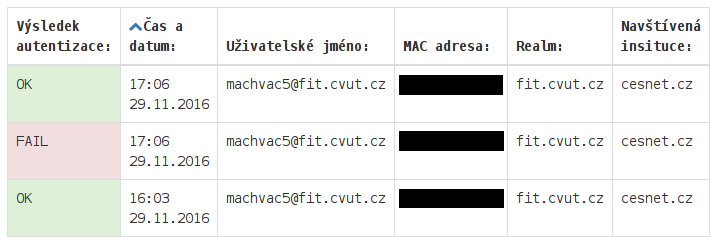
\includegraphics[scale=0.5]{search.png}
        \caption[Ukázka obecného vyhledávání]{Ukázka obecného vyhledávání}
        \label{fig:search}
      \end{figure}

      Jádrem obecného vyhledávaní rozhraní je formulář.
      Dostupná pole formuláře jsou uživatelské jméno,
      MAC adresa, výsledek autentizace, realm, navštívená instituce,
      počáteční a koncové datum a čas.
      Formulář je omezen tím způsobem, že ho nelze
      odeslat, aniž by bylo vyplněné některé z~polí,
      kromě těch, která specifikují datum a čas.
      Toto omezení je dáno rozhraním back endu pro obecné vyhledávání.

      Po odeslání formuláře jsou zobrazena nalezená data ve formě tabulky.
      Zobrazená data jsou automaticky stránkována.
      Stránkování umožňuje omezit zatížení serveru,
      protože uživatel dostává pouze část všech dostupných dat, která vyhovují parametrům dotazu.
      Rozhraní umožňuje specifikovat parametry pn a csi, 
      které jsou mapovány na uživatelské jméno a MAC adresu, pro možnosti
      předávání informací z~ostatních rozhraní front endu.
      Dostupná data jsou implicitně ražena sestupně dle časové známky událostí,
      uživatel má možnost změnit směr řazení.
      Ukázka tabulky s~nalezenými daty je na obrázku (MAC adresa je záměrně cenzurována) \ref{fig:search}.

    \subsection{Počet zařízení na uživatele}

      Rozhraní pro počet zařízení na uživatele je tvořeno
      formulářem s~poli pro počáteční a koncové datum.
      Zobrazená data jsou automaticky stránkována jako v~ostatních tabulkových rozhraních.
      Velikost stránkování je možné interaktivně definovat.
      Formulář je možné rozšířit o~dodatečné možnosti, kterými je
      uživatelské jméno a počet.
      
      U~každé dodatečné možnosti je možné specifikovat,
      jaký typ porovnání se má na zadanou hodnotu aplikovat.
      Například u~uživatelského jména může být vybrána přesná shoda nebo
      ta varianta, že uživatelské jméno obsahuje zadaný text.
      U~počtu jsou na výběr varianty rovno, větší a menší.
      U~uživatelského jména je navíc možnost vyřadit anonymní uživatele pomocí použití regulárního výrazu.
      Dodatečné možnosti vycházejí z~klíčů, které jsou definovány
      v~kolekci mac\_count, která je zdrojem dat pro toto rozhraní.
    
      Po odeslání formuláře jsou nalezená data zobrazena ve formě tabulky.
      Data jsou implicitně filtrována podle počtu zařízení bez možnosti změny.
      Zobrazená data je možné interaktivně filtrovat bez nutnosti znovu odesílat formulář.
      Lze filtrovat pomocí uživatelského jména nebo MAC adresy.
      Filtrované hodnoty jsou implicitně porovnávány na obsah uživatelského vstupu, ne na přesnou shodu.

      Pro dostatečný uživatelský komfort je možné nalezená data
      opět vyhledávat pomocí rozhraní pro obecné vyhledávání.
      Této funkcionality je dosaženo pomocí hypertextových odkazů.
      Protože jednotlivá rozhraní jsou zobrazována pomocí pohledů,
      bylo třeba nějakým způsobem předat informaci o~obsahu odkazu.

      Toho jsem docílil pomocí parametrů pohledu.
      Parametry pohledu umožňují načíst konkrétní pohled a specifikovat
      hodnoty některých proměnných.
      Pro tyto účely jsem v~rozhraní obecného vyhledávání použil parametry
      pro MAC adresu a uživatelské jméno. 
      Rozhraní je následně po kliknutí předána hodnota odkazu jako hodnota parametru.

    \subsection{Sdílená zařízení}
    
      Rozhraní pro sdílená zařízení je tvořeno
      formulářem s~poli pro počáteční a koncové datum.
      Dodatečné možnosti zahrnují MAC adresu a počet.
      Opět platí, že je možné specifikovat typ porovnání pro dodatečné možnosti.
      Stejně jako v~případě rozhraní počtu zařízení na uživatele,
      je možné nalezená data opět vyhledávat v~rozhraní pro obecné vyhledávání
      pomocí hypertextových odkazů.

      Po odeslání formuláře jsou zobrazena nalezená data ve formě tabulky.
      Data jsou implicitně řazena podle počtu uživatelů, 
      uživatel nemá možnost změnit klíč řazení ani jeho směr.
      Dostupná data je možné interaktivně filtrovat,
      filtrování je možné pomocí MAC adresy nebo uživatelského jména.
      Filtrované hodnoty jsou implicitně porovnávány na obsah uživatelského vstupu, ne na přesnou shodu.

    \subsection{Neúspěšná přihlášení}
      
      Rozhraní pro neúspěšná přihlášení je tvořeno
      formulářem s~poli pro počáteční a koncové datum.
      Po odeslání formuláře je zobrazen sloupcový graf s~daty za vybrané období.
      
      Formulář je možné rozšířit o~dodatečné možnosti, kterými je
      uživatelské jméno, počet neúspěšných přihlášení a počet úspěšných přihlášení.
      Dodatečné možnosti vycházejí z~klíčů, které jsou definovány
      v~kolekci failed\_logins, která je zdrojem dat pro toto rozhraní.
      Opět platí, že je možné specifikovat typ porovnání pro dodatečné možnosti.
      
      Toto rozhraní umožňuje jednoduchým způsobem zobrazit
      graf pro libovolnou instituci tím, že 
      v~uživatelském jméně je vyplněna pouze doménová část a je vybrán typ porovnání na obsah.
      Tato funkcionalita využívá toho, že MongoDB je schopné interně pracovat s~regulárními výrazy.

    \subsection{Uživatelé v~různých lokalitách současně}

      Rozhraní je tvořeno formulářem s~poli pro počáteční a koncové datum.
      Dodatečnými možnostmi je uživatelské jméno,
      první navštívená instituce a druhá navštívená instituce.
      Opět platí, že je možné specifikovat typ porovnání pro dodatečné možnosti.

      V~tabulce obsahující poskytovaná data jsou dostupná pole pro
      uživatelské jméno, čas obou autentizací, obě navštívené instituce,
      rozdíl časů mezi autentizacemi a čas potřebný k~přesunu mezi institucemi.
      Všechna data kromě času potřebného k~přesunu jsou získána z~kolekce logs.
      Čas potřebný k~přesunu mezi institucemi je převzat
      z~výstupu skriptu, který je popsán v~podsekci back endu \ref{concurrent_users}.
      Data jsou implicitně řazena podle uživatelského jména.

      Druhé doplňkové rozhraní je velmi jednoduché, je tvořeno pouze
      formulářem s~poli pro počáteční a koncové datum.
      Po odeslání formuláře je zobrazena tabulka, která zachycuje 
      nejčastěji vyskytující se dvojice institucí v~souvislosti
      s~uživateli v~různých lokalitách současně.
      Záznamy v~tabulce jsou řazeny podle počtu výskytů.

    \subsection{Roaming}

      Tato část textu se váže k~rozhraním organizace nejvíce poskytující konektivitu a organizace nejvíce využívající roaming.
      Rozhraní jsou totožná až na data, která zobrazují.
      Obě rozhraní jsou tvořena formulářem s~poli pro počáteční a koncové datum.
      Navíc jsou dostupné předvolby pro data za 1 měsíc, 3 měsíce a 12 měsíců.
      Dále je přítomno pole, které specifikuje počet institucí, které mají být zobrazeny.
      
      Po odeslání formuláře je zobrazen
      graf institucí seřazený podle počtu poskytnutí (nebo počtu využití v~závislosti na rozhraní).
      V~obou grafech jsou dostupné celkové počty uživatelů i počty unikátních zařízení ve vybraném období.
      Ukázka grafu organizací nejvíce poskytujících konektivitu je na obrázku \ref{fig:roaming_graph}.
      Toto rozhraní využívá data kolekce roaming pro určení celkového počtu využití nebo poskytnutí
      a data kolekce unique\_users pro určení počtu unikátních zařízení.
      
      \begin{figure}
        \centering
          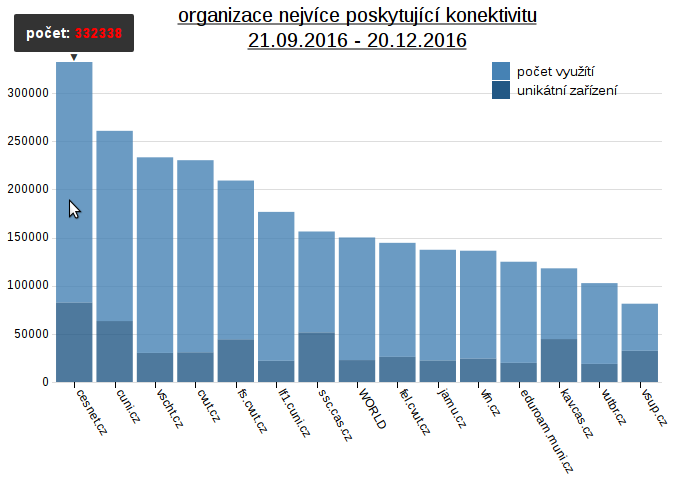
\includegraphics[scale=0.45]{roaming_graph.png}
        \caption[Ukázka grafu organizací nejvíce poskytujících konektivitu]{Ukázka grafu organizací nejvíce poskytujících konektivitu.
        Graf ukazuje data zpracovaná systémem etlog.}
        \label{fig:roaming_graph}
      \end{figure}

    \subsection{Aktivita CZ eduroamu}
    
      Rozhraní pro aktivitu CZ eduroamu je tvořeno
      formulářem s~poli pro počáteční a koncové datum.
      Navíc jsou dostupné předvolby pro data za 1 měsíc, 3 měsíce a 12 měsíců.
      Formulář je možné rozšířit o~dodatečné možnosti, kterými je realm a navštívená instituce.
      Opět platí, že je možné specifikovat typ porovnání pro dodatečné možnosti.
      Po odeslání formuláře je vykreslen graf s~daty ve vybraném období.
      Zobrazená data představují celkovou aktivitu služby v~České republice
      omezenou vstupními možnostmi.

      Zobrazovaná data jsou brána buď z~databázové kolekce roaming nebo heat\_map
      v~závislosti na tom, jak jsou vyplněna vstupní pole.
      V~případě, že není vyplněno ani jedno z~polí nebo je vyplněno jedno z~nich,
      že možné získat data z~kolekce roaming.
      Ukázka grafu je na obrázku \ref{fig:eduroam_activity}.

      \begin{figure}
        \centering
          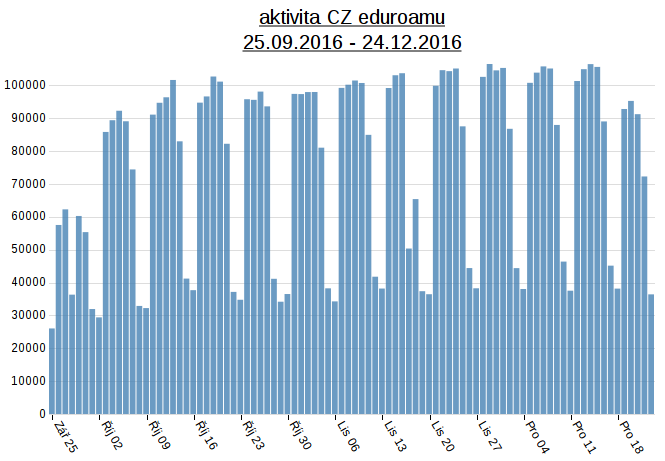
\includegraphics[scale=0.5]{eduroam_activity.png}
        \caption[Ukázka grafu aktivity českého eduroamu]{Ukázka grafu aktivity českého eduroamu. Graf ukazuje data zpracovaná systémem etlog.}
        \label{fig:eduroam_activity}
      \end{figure}

      V~případě, že uživatel chce vidět data omezená konkrétním realmem a zároveň
      navštívenou institucí, je třeba vyhledávat v~kolekci heat\_map.
      Nalezení konkrétních dat znamená dotaz na rozhraní pro mapu roamingu
      a specifikování klíčů realm a institutions.realm 
      (ke specifikování klíčů vnořených objektů se používá tečka). 
      Následně stačí určit počet přihlášení pro konkrétní instituci.

    \subsection{Mapa roamingu}

      Rozhraní pro mapu roamingu tvoří formulář
      s~poli pro počáteční a koncové datum.
      Formulář je možné rozšířit o~dodatečnou možnost, kterou je počet.
      Pro tuto možnost je dostupná pouze volba je větší.

      Omezení na počet bylo implementováno z~důvodu možnosti omezit
      mapu na instituce, které službu využívají ve výrazně větší míře než ostatní.
      Pomocí tohoto omezení je možné zkoumat pouze zlomek všech institucí.
      Omezení využívá rozhraní pro nejvíce poskytovaný a využívaný roaming
      k~určení, zda má být realm nebo navštívená instituce vyřazena.

      Před vykreslením grafu je možné navíc zvolit logaritmické měřítko.
      Tato možnost byla přidána, protože barevné spektrum grafu nebylo při jinak
      použitém lineárním měřítku dostatečně názorné.
      Pokud uživatel nevybere možnost logaritmického měřítka, je použito lineární měřítko.

      Vlastní mapa je tvořena maticí, kde řádky představují realmy a sloupce navštívené instituce.
      Mapa umožňuje interaktivní sestupné i vzestupné řazení podle řádku i sloupce,
      je opatřena interaktivními popisky pro řádky, sloupce i vlastní buňky,
      které jsou zobrazeny při pohybu kurzoru nad odpovídajícím elementem.
      Ukázka mapy roamingu je na obrázku \ref{fig:heat_map}.

      \begin{figure}
        \centering
          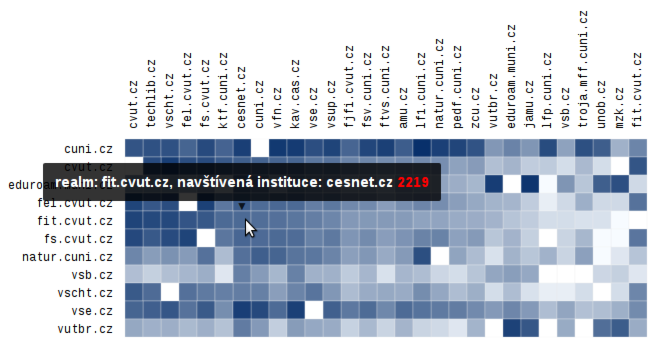
\includegraphics[scale=0.5]{heat_map.png}
        \caption[Ukázka mapy roamingu]{Ukázka mapy roamingu. Graf ukazuje data zpracovaná systémem etlog.}
        \label{fig:heat_map}
      \end{figure}

    \subsection{Počty přihlášení}

      Tato část textu se zabývá dvěma různými rozhraními, která jsou
      shodná až na data grafů.
      Tato rozhraní byla původně pouze dočasná a měla sloužit pouze pro analýzu dostupných dat.
      Výsledkem analýzy mělo být určení logiky detekující problémový stav služby
      v~některé ze zapojených institucí.
      Zadavatel definoval, že vygenerovaná data mají být ve stejné formě jako 
      data dostupná ve vizualizačních rozhraních.
      Plánoval jsem tedy využít stejný sloupcový graf, který byl použit pro ostatní rozhraní.

      Z~konzultací vyplynulo, že data mají být generována
      pro všechny české realmy.
      Pro každý realm měly být generovány tři grafy.
      První měl zobrazovat neúspěšná přihlášení
      uživatelů, druhý měl zobrazovat úspěšná přihlášení.
      Oba grafy měly být normalizovány pomocí MAC adres.
      Třetí graf měl zobrazovat data s~poměrem předchozích dvou grafů.
      Všechny grafy měly zobrazovat data za stejné časové období.

      Problémem, na který jsem oproti front endu narazil,
      bylo jak grafy generovat dávkově.
      V~případě front endu byl graf generován uživatelem po odeslání formuláře.
      Takový způsob generování dat pro tato data příliš nevyhovoval.
      Představa zadavatele byla, že všechny grafy měly být součástí
      jedné statické webové stránky.

      Pokud by byla data generována stejným způsobem jako na front endu,
      byla by data dostupná pouze uživateli, který nechal data generovat,
      případně by bylo nutné řešit přístupnost dat nějakým nestandardním způsobem.
      Po analýze možností jsem se rozhodl využít d3 jako modul back endu.

      Protože d3 je dostupný i jako modul pro Node.js,
      bylo možné i dávkové zpracování dat.
      Jelikož není při generování dostupné okno webového prohlížeče,
      byly možnosti modulu omezeny.
      Modul taktéž závisí na mnoha dalších podpůrných modulech,
      které řeší různé problémy na základě nedostupnosti webového prohlížeče.

      %Pro generování dat jsem vytvořil jednoduchý skript,
      %který využíval d3 jako back endový modul.
      %Pro samotnou logiku dotazování do databáze jsem
      %nemohl využít žádné již hotové rozhraní,
      %protože data měla být seřazena podle počtu neúspěšných přihlášení
      %pro daný realm za vybrané časové období.

      Výsledkem analýzy bylo, že data z~různých institucí byla natolik různorodá, že nebylo možné vyvodit jasný
      závěr, a zadavatel se rozhodl od této funkcionality upustit.
      Protože rozhraní bylo již hotové a poskytovalo zajímavá data v~kontextu
      funkčnosti služby, rozhraní jsem v~aplikaci ponechal a více ho zdokonalil,
      aby mohlo být v~případě nutnosti využito v~budoucnu.
 
      Obě stránky jsou generovány jednou týdně pomocí cronu.
      Pro generování jsem napsal jednoduchý Bash skript,
      který je použit pro automatické generování, ale je možné ho spustit i manuálně.
      Data grafů jsou získána z~rozhraní back endu pro kolekce visinst\_logins a realm\_logins.
      
      Rozhraní pro počet absolutních přihlášení zobrazuje počty přihlášení,
      které nejsou nijak normalizovány.
      Rozhraní s~normalizovanými počty přihlášení je normalizováno pomocí
      unikátních MAC adres v~rámci jednotlivých dnů. 
      V~tomto kontextu lze tedy o~unikátní MAC adrese uvažovat jako o~uživateli,
      ačkoliv tato rovnost nemusí vždy platit.
      
      Obě rozhraní jsou tvořena statickou webovou stránkou.
      Stránka obsahuje grafy s~daty pro 100 institucí za posledních 60 dní.
      %Pro každou instituci je dostupný graf s úspěšnými přihlášeními, 
      %graf s neúspěšnými přihlášení a graf s poměrem úspěšných a neúspěšných přihlášení.
      Pro každou instituci jsou dostupné grafy v~kontextu realmu i navštívené instituce.
      Instituce jsou seřazeny podle celkového počtu neúspěšných přihlášení v~daném období
      pro navštívené instituce.

      %Toto rozhraní bylo původně pouze dočasné a mělo sloužit pro analýzu dostupných dat.
      %Výsledky analýzy měly sloužit pro určení metody detekce nefunkčnosti služby v konkrétní lokalitě.

      %  Pro určení logiky detekující problémový stav služby
      %  bylo nejprve třeba získat podpůrná data, 
      %  ze kterých by bylo možné určit parametry detekce.
      %  Zadavatel definoval, že vygenerovaná data mají být ve stejné formě jako 
      %  data dostupná ve vizualizačních rozhraních.
      %  Použil jsem tedy stejný sloupcový graf, který byl použit pro front end.

      %  Z konzultací vyplynulo, že data mají být generována
      %  pro všechny české realmy.
      %  Pro každý realm měl být generovány tři grafy.
      %  První měl zobrazovat neúspěšná přihlášení
      %  uživatelů, druhý měl zobrazovat úspěšná přihlášení.
      %  Oba grafy měly být normalizovány pomocí MAC adres.
      %  Třetí graf měl zobrazovat data s poměrem předchozích dvou grafů.
      %  Všechny grafy měly zobrazovat data za stejné časové období.

      %  Problémem na který jsem oproti front endu narazil,
      %  bylo jak grafy generovat dávkově.
      %  V případě front endu byl graf generován uživatelem po odeslání formuláře.
      %  Takový způsob generování dat pro tato data příliš nevyhovoval.
      %  Představa zadavatele byla, že všechny grafy měly být součástí
      %  jedné statické webové stránky.

      %  Pokud by byla data generována stejným způsobem jako na front endu,
      %  byla by data dostupná pouze uživateli, který nechal data generovat,
      %  případně by bylo nutné řešit přístupnost dat nějakým nestandardním způsobem.
      %  Po analýze možností, jsem se rozhodl využít d3 jako modul back endu.

      %  Protože d3 je dostupný i jako modul pro Node.js,        % TODO - nekde drive definovat nodejs
      %  bylo možné i dávkové zpracování dat.
      %  Protože při generování není dostupné okno webového prohlížeče,
      %  byly možnosti modulu omezeny.
      %  Modul taktéž závisí na mnoha dalších podpůrných modulech,
      %  která řeší různé problém na základě nedostupnosti webového prohlížeče.

      %  Pro generování dat jsem vytvořil jednoduchý skript,
      %  který využíval d3 jako back endový modul.
      %  Pro samotnou logiku dotazování do databáze jsem
      %  nemohl využít žádné již hotové rozhraní,
      %  protože data měla být seřazena podle počtu neúspěšných přihlášení
      %  pro daný realm za vybrané časové období.

    \subsection{Stránkování}
     
      Stránkování není samostatným rozhraním, ale je součástí několika rozhraní.
      Pro stránkování jsem použil direktivu Angularu dir-paginate.
      Direktiva umožňuje specifikovat počet zobrazovaných předmětů pomocí proměnné JavaScriptu.
      Spolu s~direktivou je také dostupná HTML
      %\footnote{
      %  HTML (HyperText Markup Language) je značkovací jazyk, který se používá pro tvorbu webových stránek.
      %}
      šablona, která zobrazuje dostupné stránky.

      Při práci na stránkování mi zpočátku nebylo jasné, jak direktivu použít tím způsobem,
      aby se sama dotázala pouze na data pro konkrétní stránku.
      Tuto funkcionalitu bohužel direktiva postrádá.
      Část dotazování na data pro konkrétní stránku jsem tedy musel implementovat sám.

      Problém vznikl po zobrazení dat jedné stránky, kdy se počet předmětů na stránku
      přesně shoduje s~počtem předmětů, které poskytovalo back endové rozhraní.
      V~tomto okamžiku direktiva zafungovala tím způsobem, že nezobrazila žádné stránkování.
      Z~pohledu stránkování nebylo co stránkovat, protože byla dostupná pouze jediná stránka dat.
      
      Pro tento účel má direktiva dostupný parametr total-items, pomocí kterého je
      možné specifikovat celkový počet dostupných záznamů.
      Pro tento účel jsem využil připravené rozhraní pro stránkování,
      které vracelo přesně tuto požadovanou informaci.

  \section{Back end}
  \label{backend}
  
    Pojmem back end je označováno rozhraní aplikace,
    které poskytuje data zbylým částem aplikace.
    Back end si lze v~kontextu webové aplikace představit jako
    vrstvu mezi prohlížečem a databází,
    která se stará o~poskytování správných dat.
    
    Back end jsem strukturoval do dvou částí:
    první část je zodpovědná za zobrazování stránek ve webovém prohlížeči,
    druhá část je značně rozsáhlejší a slouží k~dotazování na data uložená v~databázi definovaným způsobem.
    Tato část je obvykle nazývána jako API\footnote{
      API (Application Programming Interface) označuje rozhraní využívané pro programování aplikací.
    }
    aplikace, protože na základě definovaného rozhraní je možné se dotazovat.

    API aplikace jsem od zbylých rozhraní oddělil pomocí cesty \verb|/api| v~URL,
    což je obvyklý způsob realizace v~současných webových aplikacích.
    Jednotlivá rozhraní jsou dále následně dostupná obvyklým způsobem.
    Rozhraní, která čerpala data z~jedné databázové kolekce
    nebo měla stejný účel, jsem vzájemně odlišil pomocí parametrů v~URL.

    Původní myšlenkou jak strukturovat samotné dotazování v~URL, bylo využít architekturu REST\footnote{
      REST (Representational state transfer) je typ architektury webových aplikací.
    }.
    REST je orientován na data aplikace, která nazývá zdroji.
    Všechny zdroje mají vlastní URL.
    REST definuje přístup ke zdrojům pomocí různých metod protokolu HTTP společně s~URL.
    Problémem, na který jsem při návrhu rozhraní pomocí architektury REST narazil,
    bylo jak reprezentovat několik nepovinných parametrů, které měly být podle definice architektury REST součástí URL.
    Parametry byly vzájemně nezávislé a mohl jich být uveden různý počet pro jeden zdroj.
    Nepodařilo se mi vytvořit strukturu, která by byla schopna reprezentovat daný zdroj
    a požadovanou operaci pomocí URL a HTTP metody.
    Z~toho důvodu jsem pro práci s~parametry zvolil query string (dotazovací řetězec).
    V~terminologii webových stránek značí query string část URL obsahující data, která nezapadají do hierarchické struktury cesty URL.

    Dotazování na back end je možné pomocí protokolu HTTP (respektive HTTPS).
    Je tedy taktéž možné využít webový prohlížeč, 
    ale vzhledem k~tomu, že jsou zobrazena pouze surová data,
    nenabízí použití webového prohlížeče žádnou potenciální výhodu.
    Pro dotazování lze však rovněž využít CLI\footnote{
      CLI (Command Line Interface) je uživatelské rozhraní, kde uživatel 
      s~programy komunikuje pomocí zapisování příkazů do příkazového řádku.  
    }
    nástroje, které jsou podle mého názoru o~mnoho vhodnější.

    Front end využívá pouze část veškerých dostupných možností dotazování back endu.
    Pomocí CLI nástrojů je možné využít veškeré možnosti, které
    rozhraní back endu nabízí.
    Pomocí CLI nástrojů lze také velmi jednoduchým způsobem dotazování automatizovat.

    Ve vlastní dokumentaci projektu je dostupných několik ukázek,
    které pro dotazování využívají nástroj cURL.
    Pomocí tohoto nástroje lze velmi jednoduchým způsobem využít veškeré
    dostupné možnosti rozhraní a díky tomu velmi přesně určit navrácená data.
    Několik pokročilých ukázek převzatých z~dokumentace
    (příkazy jsou rozděleny na více řádek z~důvodu čitelnosti):

    \begin{verbatim}
# get mac count records for 2016-10-07 with more 
# than mac addresses between 5 and 15, sort from most to least
curl 'https://etlog.cesnet.cz/api/mac_count/
?timestamp=2016-10-07&count>5&count<15&sort=-count'

# get failed logins records from 2016-09-20 to 2016-10-10 
# only for users from realm 'fit.cvut.cz'
# with no successful logins, sort from most failed logins to least
# get only 10 results
curl 'https://etlog.cesnet.cz/api/failed_logins/?
username=/.*@fit\.cvut\.cz$/&timestamp>2016-09-20&
timestamp<2016-10-10&ok_count=0&sort=-fail_count&limit=10'

# get failed logins records from 2016-09-20 to 
# 2016-09-30 only for users with realms ending '.edu'
# with fail count more than 10, sort from most to least
curl 'https://etlog.cesnet.cz/api/failed_logins/?
username=/\.edu$/&timestamp>2016-09-20&
timestamp<2016-09-30&fail_count>10&sort=-fail_count'
    \end{verbatim}

    Z~dostupných ukázek je zřejmé, že vytvořené rozhraní poskytuje
    opravdu velmi komplexní možnosti specifikace dat.
    S~využitím možnosti automatizace dotazování pomocí CLI nástrojů
    je tvorba dalších podpůrných nástrojů a následné
    dotazování na data velmi jednoduché.

    Pro všechna rozhraní, která potenciálně můžou uživateli
    poskytovat značné množství dat,
    jsem využil databázové rozhraní umožňující proudové (stream) zpracování dat.
    Toto rozhraní umožňuje definovat několik funkcí v~závislosti na stavu dat.
    Lze definovat, jaká funkce má být volána, jakmile jsou dostupná data
    nebo když jsou již zpracovány všechny záznamy.
    Právě tyto dvě možnosti jsem ve svém kódu využil.
    To mi umožnilo zpracovat libovolné množství dokumentů
    a výsledek odeslat uživateli, 
    jakmile byly všechny dokumenty zpracovány.

    Na rozdíl od způsobu zpracování
    databázových dotazů v~ostatních rozhraních
    dovoluje tento způsob pracovat s~výrazně větším množstvím dat.
    Velikost dat je v~ostatních rozhraních omezena na 16 MB.
    Přestože by se mohlo zdát, že tato velikost musí pro předávaná data postačovat,
    zdaleka tomu tak není.
    Proudové rozhraní není nijak explicitně omezeno na velikost dat,
    tudíž je velikost dat závislá na dostupných výpočetních prostředcích.

    Popis parametrů a URL všech rozhraní je dopstupný v~dokumentaci projektu
    na webové stránce \href{https://github.com/CESNET/etlog}{https://github.com/CESNET/etlog}.

    \subsection{Api-query-params}
    
      Api-query-params je modul, který jsem použil pro mapování
      query stringu na dotaz do databáze.
      Tento modul je jádrem všech rozhraní, která provádějí mapovaní query stringu na databázový dotaz.
      Jméno modulu je v~oficiální dokumentaci zkracováno na pouhé aqp, tento název budu dále v~textu používat.
      S~použitím modulu jsem vytvořil společné rozhraní, které využívají všechna rozhraní, kde je mapování třeba.

      Vlastní modul nabízí široké možnosti použití.
      Jeho největší síla spočívá v~tom, že mapuje vstup přesně na dotaz do MongoDB, 
      který již není třeba nijak dále modifikovat a je možné ho přímo použít.
      Výstupem volání modulu je objekt, který může obsahovat až několik klíčů v~závislosti
      na vstupu.

      Základním klíčem je klíč filter, který je sám objektem a obsahuje
      klíče, které odpovídají všem povoleným proměnným (kromě speciálních proměnných definujících další operátory) v~query stringu.
      Hodnoty klíčů odpovídající proměnným jsou už samotné hodnoty proměnných,
      případně může jít opět o~objekty v~závislosti na použitých operátorech.

      Dalšími klíči, které může výstup volání obsahovat, jsou sort, skip, limit a projection.
      Klíče slouží k~řazení, přeskakování, omezování počtu výsledků a projekci.
      Kromě jiného podporuje modul většinu operátorů používaných MongoDB, umožňuje specifikovat datové typy, 
      použít přetypování proměnných a taktéž dokáže pracovat s~již rozebranými objekty.
      Ukázkové použití modulu \cite{aqp} (pro názornost uvedeno na více řádcích):
      \begin{verbatim}
import aqp from 'api-query-params';
const query = aqp('status=sent&timestamp>2016-01-01
&author.firstName=/john/i&limit=100&skip=50&sort=-timestamp');
//  { 
//    filter: { 
//      status: 'sent', 
//      timestamp: { $gt: Fri Jan 01 2016 01:00:00 GMT+0100 (CET) }, 
//      'author.firstName': /john/i 
//    }, 
//    sort: { timestamp: -1 }, 
//    skip: 50, 
//    limit: 100, 
//  } 
      \end{verbatim}
      
      Všechny tyto možnosti dělají z~tohoto modulu velmi mocný nástroj,
      který jednoduše umožňuje vytvořit rozhraní, jenž definuje dotaz pomocí query stringu.
      Přesně takovouto funkcionalitu jsem do své práce potřeboval.
      Použitím tohoto modulu jsem docílil toho, 
      že rozhraní bylo tak obecné, jak umožňovala předpřipravená data.
      Uživatel následně již pouze definoval dotaz pomocí query stringu a dostal zpět data.

      Při použití modulu jsem narazil na jeden potenciální problém,
      kterým bylo použití společně s~možností whitelist.
      Whitelist v~kontextu modulu představuje možnost, kde programátor
      specifikuje, které proměnné query stringu jsou povoleny.

      Protože jsem potřeboval umožnit uživateli specifikovat pouze určité
      proměnné (vážící se na odpovídající databázovou kolekci),
      bylo nutné tuto možnost využít.
      Autor modulu měl bohužel ve svém kódu chyby, a tak bylo nutné
      ho kontaktovat a ohlásit problém. 
      Po ohlášení problému autor chyby odstranil a já jsem modul použil, jak jsem potřeboval.

      Při realizaci rozhraní používajících aqp jsem dospěl k~tomu, 
      že všechna rozhraní budou pracovat s~časovou známkou skrze query string.
      Z~toho důvodu jsem ve společném rozhraní, 
      které zapouzdřovalo aqp, vytvořil rozhraní pro ověření platné časové známky zadané uživatelem.

      Protože MongoDB je schopné pracovat s~regulárními výrazy,
      je možné je využít v~rámci celé aplikace skrze aqp.
      Regulární výraz je v~JavaScriptu řetězec z~obou stran omezený pomocí lomítek.
      Mapování obsahu proměnných v~URL, jejichž obsahem je regulární výraz, na databázový objekt probíhá právě
      tímto způsobem.

    \subsection{Obecné vyhledávaní}
    
      Obecné vyhledávací rozhraní používá aqp,
      stejně jako všechna ostatní vyhledávací rozhraní.
      Povolenými parametry query stringu je timestamp, pn, csi, visinst, realm a result,
      tedy všechny podstatné klíče databázové kolekce.

      Rozhraní je oproti ostatním specifické tím, 
      že dovoluje uživateli v~query stringu specifikovat konkrétní čas v~rámci dne.
      Důvodem pro toto je jednak užší specifikace dotazu a zároveň objem prohledávaných dat.

      Protože data v~databázi nemají žádnou vzájemnou návaznost,
      je jádrem dotazovací logiky pouze omezení uživatelským vstupem skrze aqp
      a následná projekce na všechna dostupná pole.
      Navíc může být definováno řazení, přeskakování a limit počtu výsledků.

    \subsection{Nadměrný počet zařízení}

      Povolenými parametry query stringu je username, timestamp, count a addrs.
      Parametr addrs se váže na databázový klíč addrs, který reprezentuje
      pole MAC adres zařízení jednoho uživatele.
      Pomocí aqp lze v~query stringu specifikovat více hodnot pro tento atribut zároveň.

      Problém nastává v~případě, že uživatel systému bude chtít toto
      rozhraní použít a vyhledávat podle parametru addrs, ale použije pouze jednu hodnotu.
      V~tomto případě zafunguje aqp tak, že parametr query stringu korektně přeloží
      na databázový filtr a ten se následně porovná s~hodnotou.
      Pokud by uživatel použil rovnost, tedy například \verb|addrs=12345678abcd|,
      dojde k~porovnání hodnoty konvertované na řetězec s~polem.

      Takové porovnání samozřejmě nedopadne úspěšně a uživatel se nedostane
      k~požadovaným datům, přestože mohl hodnotu adresy zadat správně.
      Přetypování hodnoty v~tomto místě nemá význam, protože s~jakýmkoliv datovým typem dopadne výsledek stejně.

      Tento problém je možné řešit pomocí databázového operátoru \verb|$in|,
      který specifikuje, že zadaná hodnota má být porovnána s prvky pole.
      Problém nespočívá v aqp, ale v tom, že
      mapování na proměnnou nemá k dispozici žádné informace o datovém typu odpovídajícího databázového klíče.

      Tento problém jsem se rozhodl řešit
      pomocí manuální konverze hodnoty na objekt reprezentující operátor \verb|$in|.
      V případě, že uživatel zadá pouze jednu hodnotu, 
      bude hodnota konvertována tím způsobem, že se porovná s každým prvkem pole relevantních záznamů.
      V případě, že uživatel zadá více hodnot, budou automaticky konvertovány pomocí aqp.
      Tímto byl tedy tento problém vyřešen.
      
      Další potíž nastala při propojení s~front endem.
      V~rozhraní front endu, používajícím toto rozhraní pro vyhledávání dat,
      byla dostupná možnost interaktivního filtrování dat,
      protože byla vstupem filtru opět pouze jedna hodnota a 
      zároveň byla tato hodnota porovnávána na částečnou shodu.
      Tudíž bylo třeba vyřešit i tento možný případ užití rozhraní.

      Prvotní implementace rozhraní narážela na problém, 
      který nastával při vyhledávání dat za časové období a ne pouze za jeden den.
      Při vyhledávání časového období mohla nastat situace, 
      kdy výsledné záznamy obsahovaly více záznamů pro stejné uživatelské jméno.
      Každý takový záznam představoval jeden konkrétní den.

      Následující implementace tento problém opravila tím způsobem,
      že všechny nalezené záznamy seskupila pomocí uživatelského jména.
      Před samotným seskupením bylo třeba ještě rozebrat pole MAC adres každého
      relevantního záznamu na jednotlivé adresy. 
      Pro tento účel jsem využil operátor \verb|$unwind|.

      Dalším problémem, který souvisí s~předchozím popsaným problémem, bylo
      omezení počtu adres.
      Omezení fungovalo správně v~případě, že se uživatel dotazoval
      na jeden konkrétní den.
      Pokud se uživatel dotazoval na data za určité časové období,
      podmínka na počet adres byla uplatněna hned v~úvodní fázi filtrování dat.

      Protože data jsou v~databázi uložena po jednotlivých dnech,
      znamenalo to, že podmínka na počet byla uplatněna na každý jednotlivý záznam,
      který vyhovoval vybranému časovému intervalu.
      Tento přístup byl samozřejmě chybný, a tak mohl uživatel dostat data, která nevyhovovala
      dané podmínce.
      Řešením tohoto problému bylo odstranit podmínku z~úvodního filtrování
      a aplikovat ji až po seskupení všech záznamů podle uživatelského jména.

    \subsection{Sdílená zařízení}
    
      Povolenými parametry query stringu je timestamp, count, mac\_address a users.
      Stejně jako v~případě nadměrného počtu zařízení je 
      v~databázové kolekci, která je spojena s~rozhraním, přítomný klíč, jehož datovým typem je pole.
      Problémy, na které jsem narazil v~případě nadměrného počtu zařízení jsem v~tomto rozhraní řešil stejným způsobem.

    \subsection{Neúspěšná přihlášení}
      
      Povolenými parametry query stringu je username, timestamp, fail\_count, ok\_count a ratio.
      Stejně jako v~případě ostatních rozhraní bylo třeba brát v~potaz případ, 
      kdy bude rozhraní dotázáno na časové období.

      Dotaz na časové období znamenal, že výsledné záznamy musely být seskupeny podle uživatelského jména,
      a podmínky na klíče fail\_count, ok\_count a ratio musely být aplikovány až po tomto seskupení.
      Seskupení záznamů taktéž znamenalo, že musely být přepočteny hodnoty klíčů fail\_count, ok\_count a ratio.

      Získat výsledné hodnoty ok\_count a fail\_count bylo snadné -- šlo o~součet hodnot ve všech záznamech
      se stejným uživatelským jménem.
      Výsledná hodnota ratio závisela na předchozích dvou. 
      V~tomto případě bylo nutné využít operátory pro součet a dělení.

    \subsection{Roaming}

      Pro roamingová data jsou dostupná dvě samostatná rozhraní.
      Rozhraní jsou si vzájemně velmi podobná a liší se pouze v~několika drobných detailech.
      V~obou rozhraních jsou pro query string povoleny parametry timestamp, inst\_name, provided\_count a used\_count.
      Rozhraní poskytují data o~počtech unikátních zařízení v~kontextu poskytování a využívání roamingu.

    \subsection{Mapa roamingu}

      Povolenými parametry query stringu pro rozhraní mapy roamingu je timestamp, realm, institutions.realm a institutions.count
      (notací pro přístup k~položkám vnořených objektů je tečka).
      Dotazovací logika tohoto rozhraní je založena na dotazu pro interval.
      Pro tento dotaz bylo třeba výstup upravit takovým způsobem,
      že každá instituce jako realm měla být ve výstupu uvedena pouze jednou.
      Pro dosažení takového výstupu muselo být nejdříve rozloženo pole institutions,
      následně byly záznamy seskupeny podle realmu a jména instituce, která realm navštívila, 
      společně se seskupením byl uložen počet záznamů, který odpovídal počtu navštívení.
      Následně stačilo pouze seskupit záznamy podle realmu a přidat všechny instituce do pole společně s~počtem.

    \subsection{Přihlášení v~realmech a navštívených institucích}
      Tato část textu se zabývá dvěma rozhraními, která
      realizují stejnou funkcionalitu.
      Rozdílem mezi rozhraními jsou data, která vracejí -- jde buď
      o~informace o~přihlašování uživatelů v~realmech nebo v~navštívených institucích.

      Tato rozhraní můžou být považována pouze za doplňková,
      protože nejsou přímo vázána na žádná rozhraní front endu pomocí formulářů.
      Rozhraní jsou využita pro generování grafů počtů přihlášení,
      které jsou dostupné jako součást front endu.
      Toto rozhraní front endu mělo být pouze dočasné, 
      ale bylo rozhodnuto, že bude zachováno, proto jsem ponechal i tuto část rozhraní back endu.

      Data pro grafy byla původně získávána z~rozhraní pro neúspěšná přihlášení
      a z~rozhraní pro úspěšná přihlášení.
      Obě rozhraní pracovala se seskupováním záznamů pomocí uživatelských jmen.
      Tento přístup je naprosto v~pořádku, vyžaduje však vysokou kvalitu zdrojových dat,
      která nemusí být vždy dostupná.

      Logika dotazování na konkrétní instituce byla realizována pomocí
      regulárního výrazu, kde byla vyplněna pouze doménová část.
      Tento regulární výraz byl obsahem parametru pro uživatelské jméno.
      V~případě, že zdrojová data nebyla dostatečně kvalitní, mohl mít tento přístup 
      velmi špatné důsledky na výsledná data.
      V~případě, že některá instituce neměla uživatelská jména svých uživatelů vyplněna
      nebo je měla vyplněna jen v~některých případech, značně to ovlivnilo kvalitu výsledných dat.

      Z~toho důvodu jsem se rozhodl od tohoto přístupu upustit a pracovat pouze
      s~realmem či navštívenou institucí, které jsou vždy vyplněny.
      Tento přístup se ukázal jako o~mnoho vhodnější. 
      Z~toho důvodu jsem použil rozhraní, která používají tento přístup.
      Rozhraní pro úspěšná přihlášení nemělo nadále v~aplikaci žádný význam, 
      proto jsem toto rozhraní odstranil.

    \subsection{Unikátní uživatelé}
      
      Povolenými parametry query stringu je timestamp a realm.
      Rozhraní vrací požadovaná data na základě parametru dotazu, který je součástí URL.
      Parametrem je buď realm nebo visinst.
      V~závislosti na hodnotě parametru poskytuje rozhraní data
      pro realm nebo navštívenou instituci daného jména.
      
      Ačkoliv je rozhraní nazváno unique\_users (unikátní uživatelé),
      poskytuje informace o~počtech unikátních zařízení.
      V~textu je již několikrát zmíněno, že o~unikátních
      zařízeních je možné uvažovat jako o~unikátních uživatelích s~určitou mírou nepřesnosti.
      Jádrem dotazovací logiky tohoto rozhraní je práce s~poli MAC adres,
      které je nejdříve rozloženo, následně jsou záznamy seskupeny podle realmu
      a všechny adresy jsou opět přidány do pole.
      Posledním krokem je výpočet délky pole.

    \subsection{Souběžní uživatelé}
    \label{concurrent_users}
      
      Zdrojová data pro toto rozhraní jsou získána z~XML\footnote{
        XML (Extensible Markup Language) je obecný značkovací jazyk, který definuje sadu pravidel
        pro kódování dokumentů do formátu, který je čitelný pro lidi i počítače.
      }
      dokumentu, ve kterém jsou obsaženy informace o~všech zapojených institucích z~České republiky.
      Pro každou instituci je uveden seznam bodů ve kterých je eduroam nasazen včetně
      geografických informací.
      Samotné záznamy neobsahují informaci o~tom, ze kterého bodu dané instituce autentizace vzešla.
      Ukázka mapy pokrytí je na obrázku \ref{fig:geo_map}.

      \begin{figure}
        \centering
          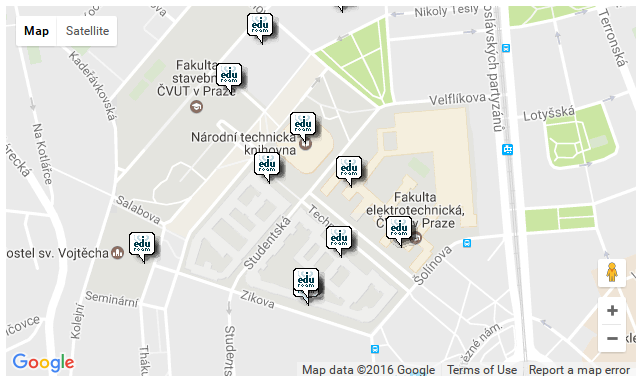
\includegraphics[scale=0.5]{geo_map.png}
        \caption[Ukázka pokrytí služby eduroam]{Ukázka pokrytí služby eduroam \cite{eduroam_cz}}
        \label{fig:geo_map}
      \end{figure}


      Geografické informace jsou zpracovány pomocí transformačního skriptu.
      Autorem skriptu je Ing. Jan Tomášek.
      Postup zpracování je možné popsat následujícím způsobem:
      skript porovná všechny body každé instituce,
      pro každou dvojici institucí najde takové body,
      které jsou si nejblíže a z~jejich vzdáleností spočte nejkratší čas, 
      ve kterém se uživatel může přesunout při dané rychlosti.
      Výstupem je matice všech institucí, 
      kde pro každou dvojici je uvedena vzdálenost dvou nejbližších bodů a čas potřebný k~přesunu.
      Výstupním formátem skriptu je formát JSON.
     
      %Geografické informace jsou využity takovým způsobem,
      %že pro každou z institucí je vypočten průměr ze vzdáleností všech dostupných bodů.
      %Pro všechny body instituce je určena vzdálenost od tohoto průměru.
      %Ze vzdáleností je určeno maximum.
      %
      %Pokud nejsou body instituce příliš vzdálené (Konkrétní mez je definována ve zdrojovém kódu),
      %je instituce přidána do výstupního seznamu.
      %Instituce, které mají jednotlivé body dále než je definovaná mez nejsou vůbec brány v potaz.
      

% Delam to ze spocitam prumer ze vsech bodu instituce a pak vzdalenost vsech bodu od tohoto prumeru a urcim si maximum techto vzdalenosti. Pokud neni instituce rozlezla, treba jako vutbr.cz tak vyleze relativne mala vzdalenost - 2833m. Kdyz ma nejaky body daleko, treba jako vsb.cz ma pracoviste v moste, tak tam mame 321km tak bohuzel tuhle instituci vubec nebereme v potaz.

% I tech 2833m VUT je hodne. Ale je nutny pocitat s tim ze data nejsou presny a tak se musime vzdat zachytavani incidentu v tom samem meste. Smerujeme k tomu chytat lidi kteri se fakt rychle objevi v jinem meste.


% Pouzil jsem inteligentnejsi algoritmus. Pracuje se vsemi body kazde instituce. Pro kazdou dvojici instituci najde takove body ktere jsou si nejbliz a z jejich vzdalenosti spocte nejkratsi cas ve kterem se uzivatel muze presunout. Napr. cesnet.cz a cuni.cz maji vzdalenost jen 0.5km (mame pokryty hlavak), cesnet.cz a vsb.cz jen 70km (VSB ma neco v moste). Takze neni treba vytridit instituce ktere jsou prilis rozlezle a mame tak vetsi sanci nekoho odchytit.


      %Tuto funkcionalitu realizuje transformační skript.
      %Všechny instituce, které splňují podmínku jsou následně
      %vypsány ve formátu JSON.

      Výstup skriptu je následně již zpracován pomocí denní periodické úlohy, která je součástí aplikace.
      Logika zpracování výstupu je následující:
      pro každou rozdílnou dvojici institucí je pro daný den
      nalezen seznam uživatelů, kteří navštívili obě zpracovávané instituce.
      Služba eduroam umožňuje používat takzvanou anonymní identitu, kde není specifikováno jméno uživatele.
      Tato funkcionalita představovala v~tomto kontextu uživatele, kteří se mohli vyskytovat souběžně
      v~několika různých institucích. Z~toho důvodu bylo třeba anonymní uživatele vyřadit.
      
      Pro každého uživatele v~tomto seznamu je následně provedeno vyhledávání
      pro obě zpracovávané instituce.
      Záznamy jsou následně iterovány.
      Při změně navštívené instituce v~aktuálním záznamu oproti předchozímu
      je porovnán čas autentizace obou záznamů a pokud je menší,
      než čas potřebný k~přesunu, jsou tyto dva záznamy sloučeny do jednoho a uloženy.

      Rozhraní tedy poskytuje data o~uživatelích, kteří
      se úspěšně ověřili v~různých institucích v~čase, který je kratší,
      než by měl být podle vypočtených dat o~pokrytí služby.
      Povolenými parametry query stringu je timestamp, username, visisnt\_1 a visisnt\_2.

    \subsection{Souběžné instituce}
      
      Rozhraní pro souběžné instituce poskytuje data
      za vybrané časové období o~nejčastěji se vyskytujících dvojicích institucí,
      kde se souběžně vyskytují uživatelé.
      Rozhraní využívá data kolekce concurrent\_users.
      Povoleným parametrem query stringu je pouze timestamp.

      Při implementaci rozhraní jsem nebyl schopen navrhnout databázovou logiku,
      která by byla schopna seskupit dvojice stejných navštívených institucí
      s~rozdílným pořadím.
      Tuto funkcionalitu jsem realizoval v~rozhraní front endu.

    \subsection{Stránkování}
       
       Rozhraní pro stránkování je navrženo tím způsobem,
       že jako parametr požaduje název kolekce. 
       Dalším povinným vstupem je omezení časové známky
       v~query stringu, zbytek je již volitelný.

       Toto rozhraní má pouze jediný účel, kterým je získat celkový
       počet záznamů pro konkrétní dotaz na jiné rozhraní.
       Pomocí této informace je front end schopen stránkovat
       nalezená data.

       Pro jednotlivé parametry, kterými jsou názvy rozhraní, 
       jsem vytvořil samostatné funkce,
       které používají velmi obdobnou logiku jako samotná rozhraní.
       Bylo třeba dodat jednoduchou logiku, 
       která k~dřívější funkcionalitě přidává celkový počet záznamů.

    \subsection{Ostatní rozhraní}
      
      Ostatní rozhraní plní především podpůrnou roli pro hlavní rozhraní a front end.

      Důležitým rozhraním je rozhraní db\_data. 
      Rozhraní nepřijímá žádný vstup, jeho výstupem je objekt
      s~klíči odpovídajícími všem kolekcím, 
      které obsahují časové známky.
      Data každého klíče jsou opět objekty, ty už ale obsahují pouze klíče min a max, 
      kde v~každém klíči je uložena minimální (nebo maximální) hodnota
      časové známky, pro kterou jsou data odpovídající kolekce dostupná.
      
      Dalším podpůrným rozhraním je rozhraní realms.
      Rozhraní nepřijímá žádný vstup, jeho výstupem
      je abecedně seřazený seznam realmů v~České republice.
      Pro účely autentizace je dostupné podpůrné rozhraní, které
      poskytuje metadata pro protokol SAML\footnote{
        SAML (Security Assertion Markup Language) je otevřený standard založený na XML, 
        který slouží pro výměnu autorizačních a autentizačních informací mezi dvěma entitami, obvykle IdP a SP.
        Protokol SAML je definován v~RFC 7522.
      }.

    \subsection{Periodické úkony}

      Stejně jako v~operačním systému jsem v~aplikaci pro realizaci periodických úkonů použil cron.
      Samozřejmě byl reprezentován modulem back endu.
      Úlohy byly separovány z~důvodu závislosti na databázi.
      Úlohy jsou definovány následovně:

      \begin{center}
        \begin{tabular}{ | c | c | }
          \hline
             čas spuštění                 & popis úlohy                            \\ \hline
             první den v~měsíci v~06:00   & report o~neúspěšných přihlášeních      \\ \hline
             každý den v~02:05            & výpočet dat kolekce failed\_logins     \\ \hline
             každý den v~02:15            & výpočet dat kolekce mac\_count         \\ \hline
             každý den v~02:20            & výpočet dat kolekce roaming            \\ \hline
             každý den v~02:25            & výpočet dat kolekce shared\_mac        \\ \hline
             každý den v~02:35            & výpočet dat kolekce realm\_logins      \\ \hline
             každý den v~02:40            & výpočet dat kolekce visinst\_logins    \\ \hline
             každý den v~02:45            & výpočet dat kolekce heat\_map          \\ \hline
             každý den v~02:55            & výpočet dat kolekce unique\_users      \\ \hline
             každý den v~03:00            & odstranění starých dat kolekce logs    \\ \hline
             každý den v~03:10            & výpočet dat kolekce concurrent\_users  \\ \hline
             každých 15 minut             & výpočet dat kolekce users\_mac         \\
          \hline
        \end{tabular}
      \end{center}

    \subsection{Podpůrné skripty}
      
      Pro práci systému byla potřeba celá řada podpůrných skriptů.
      Skripty pro transformaci dat a jejich import jsem popsal podrobně v~sekci \ref{logs_processing}.
      Skript pro transformaci geografických dat o~pokrytí služby je popsán v~podsekci \ref{concurrent_users}.
      Ostatní podpůrné skripty jsou popsány dále.


      %\subsubsection{Detekce stavu služby}
      %  Pro určení logiky detekující problémový stav služby
      %  bylo nejprve třeba získat podpůrná data, 
      %  ze kterých by bylo možné určit parametry detekce.
      %  Zadavatel definoval, že vygenerovaná data mají být ve stejné formě jako 
      %  data dostupná ve vizualizačních rozhraních.
      %  Použil jsem tedy stejný sloupcový graf, který byl použit pro front end.

      %  Z konzultací vyplynulo, že data mají být generována
      %  pro všechny české realmy.
      %  Pro každý realm měl být generovány tři grafy.
      %  První měl zobrazovat neúspěšná přihlášení
      %  uživatelů, druhý měl zobrazovat úspěšná přihlášení.
      %  Oba grafy měly být normalizovány pomocí MAC adres.
      %  Třetí graf měl zobrazovat data s poměrem předchozích dvou grafů.
      %  Všechny grafy měly zobrazovat data za stejné časové období.

      %  Problémem na který jsem oproti front endu narazil,
      %  bylo jak grafy generovat dávkově.
      %  V případě front endu byl graf generován uživatelem po odeslání formuláře.
      %  Takový způsob generování dat pro tato data příliš nevyhovoval.
      %  Představa zadavatele byla, že všechny grafy měly být součástí
      %  jedné statické webové stránky.

      %  Pokud by byla data generována stejným způsobem jako na front endu,
      %  byla by data dostupná pouze uživateli, který nechal data generovat,
      %  případně by bylo nutné řešit přístupnost dat nějakým nestandardním způsobem.
      %  Po analýze možností, jsem se rozhodl využít d3 jako modul back endu.

      %  Protože d3 je dostupný i jako modul pro Node.js,        % TODO - nekde drive definovat nodejs
      %  bylo možné i dávkové zpracování dat.
      %  Protože při generování není dostupné okno webového prohlížeče,
      %  byly možnosti modulu omezeny.
      %  Modul taktéž závisí na mnoha dalších podpůrných modulech,
      %  která řeší různé problém na základě nedostupnosti webového prohlížeče.

      %  Pro generování dat jsem vytvořil jednoduchý skript,
      %  který využíval d3 jako back endový modul.
      %  Pro samotnou logiku dotazování do databáze jsem
      %  nemohl využít žádné již hotové rozhraní,
      %  protože data měla být seřazena podle počtu neúspěšných přihlášení
      %  pro daný realm za vybrané časové období.

      \subsubsection{Invalidní záznamy}

        Odkazy na soubory obsahující invalidní záznamy v~reportu
        byly další částí, kterou bylo třeba řešit.
        Chybovým výstupem transformačního skriptu byly řádky
        problémových záznamů společně s~důvodem, proč byl daný záznam považován za invalidní.
        Tyto informace bylo třeba využít k~získání původních záznamů a umístit je do příslušných souborů.

      \subsubsection{Zpracování historických dat}
        
        Historická data, která byla importována do databáze,
        představovala pouze samotné záznamy kolekce logs.
        Ze záznamů byla periodicky předpočítávána
        data ostatních kolekcí.
        Z~toho důvodu jsem pro předpočítávání historických
        dat ostatních kolekcí vytvořil samostatný skript.
        Skript využívá logiku pro zpracování aktuálních dat,
        pouze specifikuje jiné časové intervaly.

      \subsubsection{Archivace}
        
        Z~důvodu redukce zabraného diskového
        prostoru historickými soubory jsem
        vytvořil archivační skript, který je automaticky spouštěn jednou týdně.
        Skript archivuje soubory s~invalidními záznamy,
        soubory s~chybovým výstupem transformace dat a samotné F-Ticks log soubory.
        Tyto soubory představují největší část zabíraného místa vyjma databáze.
        Žádné soubory nejsou mazány, tato činnost
        je potenciálně ponechána na správci aplikace v~případě nedostatku diskového prostoru na serveru.

    \section{Autentizace}
      
      Přestože autentizace nebyla součástí zadaní diplomové práce,
      z~povahy dostupných dat bylo zřejmé, že bude třeba zabezpečit přístup k~systému,
      aby nebyla data dostupná komukoliv.
      V~případě, že by systém nebyl nijak zabezpečen, bylo by pro kohokoliv v~Internetu možné
      k~němu přistoupit a získat data, která obsahuje.

      Původním návrhem bylo realizovat autentizaci pomocí České akademické federace identit eduID.cz.
      Cílem této federace je poskytnout svým členům rámec pro vzájemné využívání
      identit uživatelů při řízení přístupu k~síťovým službám.
      Výhody federace\cite{eduid_cz}:
      
      \begin{itemize}
        \item{uživatel používá pouze jedno heslo pro přístup k~více aplikacím,}
        \item{správci aplikací neudržují autentizační data uživatelů, ani neprovádí autentizaci,}
        \item{autentizace uživatele probíhá vždy v~kontextu domovské organizace, citlivé autentizační údaje uživatele neopouští domovskou síť,}
        \item{federační infrastruktura poskytuje snadný, standardní a bezpečný způsob výměny informací o~uživatelích.}
      \end{itemize}

      Federace eduID.cz je postavena na projektu Shibboleth. 
      Shibboleth je implementací protokolu SAML.
      Vzájemná komunikace mezi SP i IdP tedy probíhá pomocí protokolu SAML.
      Z~toho důvodu bylo nutné do aplikace dodat logiku, která by takovou komunikaci realizovala\cite{eduid_cz}.

      Pro tento účel jsem v~aplikaci využil knihovnu Passport společně s~modulem
      passport-saml.
      Modul passport-saml je implementací protokolu SAML v~JavaScriptu.
      V~jeho oficiální dokumentaci je uvedeno, že je kompatibilní s~projektem Shibboleth.

      Konfigurace samotného modulu byla velice složitá,
      kvůli nekvalitní dokumentaci.
      Pro účely ladění procesu konfigurace společně s~testováním autentizace
      byla aplikace napojena na testovací IdP (nebo testovacího poskytovatele identity).
      Pro účely implementace autentizace mi byl taktéž vytvořen uživatelský účet.

      Samotné přesměrování na autentizační server i zpět do aplikace
      probíhalo korektně.
      Při návratu do aplikace jsem však narazil na chybové hlášení.
      Problémem bylo, že toto chybové hlášení se zobrazovalo
      pouze při snaze autentizovat v~rámci aplikace mě přiděleného uživatele,
      ostatní uživatelé na tento problém nenaráželi.

      Zadavatel rozhodl, že řešení tohoto problému mám ponechat na něm.
      Důvodem byla implementace zbylých částí systému a omezený přístup
      k~log souborům testovacího federačního serveru, které mohly pomoci s~laděním problému.
      Před dokončením implementace se bohužel nepodařilo
      tento problém nijak vyřešit.

      Protože autentizaci se nepodařilo tímto způsobem realizovat, navrhl jsem nové jednodušší řešení.
      Řešením bylo použít nástroj iptables tak,
      že mohly do aplikace přistupovat pouze definované zdrojové IP adresy.
      Ačkoliv toto řešení neposkytuje samo žádnou formu autentizace,
      spolehlivě dokáže zamezit přístupu do aplikace.
      Návrh tohoto řešení byl přijat a nasazen.

    \section{Analýza dat}
      
      Analýzu dostupných dat bylo třeba provádět ještě před započetím implementace
      a taktéž v~jejím průběhu.
      Provádět analýzy ručně nad obsahem dat databáze bylo zdlouhavé,
      proto jsem se k~tomuto řešení uchyloval až jako k~poslední možnosti.
      V~průběhu implementace webového rozhraní bylo již možné provádět
      analýzy různých dat dostupných v~systému, což bylo o~mnoho vhodnější.

      Pomocí dat dostupných v~reportech s~invalidními záznamy se podařilo
      snížit počty invalidních záznamů z~více než 20 \% v~průměru pro jeden den na přibližně 1 \%.
      Tato analýza tedy podle mého názoru pomohla velmi výrazně zlepšit kvalitu
      vstupních dat.
      Stále však zůstává mnoho institucí, kde není vůbec vyplněno uživatelské jméno
      nebo je vyplněno nesprávným způsobem.

      Pomocí dat dostupných skrze rozhraní pro nadměrný počet zařízení se
      podařilo odhalit dvě identity, které zahrnovaly více než 100 zařízení.
      Zadavatel při komunikaci se zodpovědnými IdP zjistil, 
      že se jednalo účty, 
      které byly poskytovány návštěvníkům v~rozporu s~pravidly eduroamu. 
      Odhalení takových účtů a zajištění nápravy by bez mého systému bylo mnohem obtížnější.
      
      Data dostupná v~tomto rozhraní zahrnují mnoho dalších identit, které
      jsou spojeny s~vysokými počty zařízení.
      Je obtížné určit, zda jsou tyto identity kompromitovány,
      protože moderní operační systémy poskytují uživatelům
      možnost randomizace MAC adres.
      To znamená, že uživatel je schopen vygenerovat mnoho legitimních
      záznamů s~různými MAC adresami, a přesto nebude jeho identita kompromitována.

      Pro analýzu toho, zda uživatel používá tuto funkcionalitu nebo zda jde
      o~kompromitovanou identitu, by musela být funkcionalita rozhraní rozšířena.
      Rozšíření by mělo být založeno na zkoumání toho, kdy byly
      jednotlivé MAC adresy aktivní.

      Toto rozšíření bohužel samo o~sobě taktéž nestačí,
      protože uživatel může službu eduroam využívat na více zařízeních současně.
      Tato funkcionalita by musela být navíc rozšířena takovým způsobem,
      aby poskytovala data pouze o~uživatelích, 
      kteří by měli současně aktivních několik MAC adres.

      Na základě takového rozšíření by bylo možné vyřadit uživatele, 
      kteří využívají randomizaci MAC adres.
      Odhalení kompromitovaných identit by mohlo být ale stále problematické,
      protože by bylo nutné určit mez počtu zařízení,
      která můžou být současně aktivní.
      Je zřejmé, že někteří uživatelé mohou mít aktivních současně
      několik zařízení a jejich identita nebude kompromitována.
      Jiné identity můžou být naopak kompromitovány, 
      ale může se jednat pouze o~dvě nebo tři různá zařízení.

      Analýzy dat v~rozhraních, ve kterých se pracuje se seskupováním
      pomocí uživatelského jména, ukázaly, 
      že instituce, které uživatelské jméno nevyplňují, můžou způsobit různé druhy problémů.
      V~případě, že instituce nevyplňuje uživatelské jméno vůbec, 
      nelze pro tuto instituci provádět určité typy analýz.
      V~případě, že je v~některých případech jméno vyplněno a v~některých
      případech není, 
      může dojít k~vygenerování dat, která budou poskytovat velmi nepřesné výsledky.

      Analýza dat současně se vyskytujících uživatelů ukázala na instituce, 
      které poskytují neaktuální informace o~pokrytých lokalitách. 
      Můj systém následně chybně detekuje uživatele, 
      kteří se mezi institucemi přesouvají příliš rychle, 
      protože nejsou dostatečné informace o~pokrytých lokalitách. 
      Přes nedostatečnost podkladů dokázal můj systém detekovat 
      několik uživatelů, jejichž identita byla kompromitována. 
      Pro potvrzení správnosti bylo nutné, aby zadavatel kontaktoval 
      instituce, kde se kompromitovaní uživatelé připojili, a ověřil, 
      kde se uživatel skutečně připojil.
      Potvrzené kompromitované identity byly předány k~dalšímu řešení bezpečnostním týmům.

      Pro podporu zlepšení informací o~pokrytí eduroamem 
      jsem implementoval rozhraní, 
      které hlásí takové kombinace institucí, 
      mezi kterými dochází k~velmi rychlým přesunům příliš často, 
      a tudíž pravděpodobně poskytují nekompletní informace. 
      Na základě těchto informací začal zadavatel s~dotčenými institucemi jednat o~doplnění dat. 
      To vede k~zlepšení poskytovaných dat a zlepšení přesnosti detekce.

      % Analýza dat současně vyskytujících se uživatelů ukázala,
      % že některé instituce mají nepřesně vyplněné informace o~svém pokrytí.
      % Na základě této analýzy se podařilo některé z~institucí donutit,
      % aby informace aktualizovaly nebo dodaly správné informace o~pokrytí.

      Součástí zadání diplomové práce měla být taktéž implementace detekce
      současně se vyskytujících zařízení.
      Stejně jako v~případě souběžně vyskytujících se uživatelů by mělo jít
      o~zařízení, která se vyskytují v~krátkém časovém intervalu v~různých navštívených institucích.
      Společně se zadavatelem jsme dospěli k~názoru, že při vyloučení dat současných uživatelů
      by data současně vyskytujících se zařízení mohla představovat dva typy uživatelů.

      Mohlo by jít o~uživatele, kteří využívají randomizace MAC adres nebo
      používají jinou MAC adresu, než je fyzická adresa zařízení.
      Ani jeden z~těchto případů nepřinášel žádná opravdu podstatná data.
      Spolu se zadavatelem jsme dospěli k~názoru, že tato data by v~systému nebyla naprosto nijak přínosná.
      Z~toho důvodu zadavatel zrušit požadavek na tuto funkcionalitu.
      
      Z~reportů o~neúspěšných přihlášeních vyplynulo,
      že mnoho uživatelských jmen, 
      která se pohybují u~vrcholu žebříčku v~počtu neúspěšných přihlášení,
      používají doménové jméno \verb|wlan.mnc003.mcc230.3gppnetwork.org| nebo nějaké velmi podobné.
      Jedná se o~automatickou konfiguraci některých zařízení, 
      která se pokoušejí připojit k~bezdrátové síti a používají identity s~touto doménou.

      Analýza dat o~počtech přihlášení byla velmi zdlouhavá a náročná.
      Pro většinu institucí, které poskytovaly nebo využívaly službu ve velké
      míře (řádově tisíce unikátních uživatelů denně),
      byly v~grafech na první pohled zřejmé výkyvy, které tvořily víkendy.
      
      Data všech institucí byla vzájemně velmi různorodá,
      přesto byla společným rysem podobná data grafu, který
      zachycoval poměr úspěšných a neúspěšných přihlášení.
      Data většiny institucí se pohybovala na ose y v~průměru kolem hodnoty 6 pro normalizovaná data.
      Existovaly samozřejmě i instituce, které dosahovaly výrazně malých i velkých hodnot.
      Tato data v~praxi znamenala, že na 6 úspěšných přihlášení připadá jedno neúspěšné přihlášení.
      Jeden z~dřívějších incidentů s~funkčností služby,
      který byl zachycen v~grafech, měl být vodítkem pro určení metody detekce problémového stavu služby.
      Bohužel ani toto vodítko nijak nepřispělo k~určení metody.

      Jak jsem již napsal, moderní operační systémy
      poskytují uživatelům možnost randomizovat MAC adresy zařízení.
      Uživatelé, kteří využívají tuto možnost, mohou zhoršit výsledky dostupných analýz.
      Například z~pohledu úspěšných či neúspěšných přihlášení
      může takový uživatel statistiky různě ovlivnit.
      Z~dostupných analýz vyplynulo, že uživatelů služby,
      kteří tuto funkci využívají, není mnoho,
      přesto mohou působit určité potíže.

\begin{conclusion}

  Diplomová práce byla vytvořena na základě spolupráce Fakulty informačních technologií
  Českého vysokého učení technického v~Praze a sdružení CESNET za účelem vylepšení služby eduroam.
  Pro vývoj systému bylo třeba se seznámit s~danou problematikou a získat vhled do fungování celého procesu.
  V~průběhu vývoje bylo mnoho součástí systému několikrát přepracováno na základě konzultací a požadavků zadavatele.
  Cílem práce bylo vytvořit systém, který by umožňoval sledovat stav služby,
  provádět různá vyhledávání a detekovat anomálie týkající se této služby.
  Podařilo se mi vytvořit systém pro analýzu roamingového systému eduroam a tím splnit zadání diplomové práce.
  Vytvořený systém je podle mě velmi obecně koncipován, co se týče možností vyhledávání.
  Všechna rozhraní, která umožňují vyhledávat a používají modul api-query-params, může
  uživatel využít pro dotaz na téměř libovolná data.

  Stav sběru logů před započetím implementace byl prováděn ve dvou formách -- v~úplné a v~redukované.
  Úplná forma log souborů je tvořena laděním obsahu procházejících EAP paketů.
  Kvůli své informační hodnotě je tato forma log souborů vhodná pro podrobnou
  analýzu jednotlivých paketů, ta je však velmi časově náročná a vyžaduje detailní znalosti protokolu.
  Redukovaná forma log souborů je výrazně méně obsáhlá. 
  Každý záznam je tvořen pouze několika klíčovými atributy.
  Log soubory jsou generovány pomocí RADIUS serveru.

  Věřím, že zpracování logů je provedeno precizně. 
  Systém provádí vše od filtrace vstupních hodnot přes import do databáze až pro výpočet podpůrných dat pro analýzy.
  Filtrace vstupních hodnot kontroluje správný počet všech atributů, které mají být definovány,
  stejně tak je kontrolován jejich obsah.
  Vstupní hodnoty jsou následně konvertovány do databázového formátu a importovány.
  Následné prováděné analýzy kompletně definoval zadavatel, 
  proto nemusí být zcela obecné, přesto jsem se při implementaci snažil, aby mohly být jejich výsledky jak obecné, tak konkrétní.

  Statistiky jsou jednou z~důležitých součástí systému a jsou v~systému dostupné skrze grafy a reporty.
  Grafy je možné generovat na několika různých rozhraních.
  Na každém z~rozhraní je možné graf blíže určit pomocí vstupních parametrů,
  a tak jsou mohou být výsledné statistiky přesně uzpůsobeny uživatelovým potřebám.
  V~reportech jsou dostupné informace o~záznamech za poslední interval
  v~závislosti na typu reportu.

  Reporty jsou řešeny pomocí emailů.
  Původně měl systém poskytovat 3 různé druhy reportů, ale kvůli nejasné metodě,
  která by určila problémový stav služby, 
  byl tento typ reportu zadavatelem zrušen.
  Systém poskytuje reporty o~invalidních záznamech a reporty o~neúspěšných přihlášeních.
  Adresáti reportů jsou určování na základě obsahu databáze,
  je tedy možné je měnit bez zásahu do zdrojových kódů systému.
  Reporty o~neúspěšných přihlášeních taktéž poskytují funkcionalitu
  pro notifikaci správců jednotlivých institucí včetně odpovídajících dat.

  Analýza trendů, které mohou signalizovat nefunkčnost služby,
  měla být původně zpracována jako jeden z~reportů.
  Analýza podpůrných dat ukázala, 
  že nelze určit spolehlivou metodu pro detekci problémového stavu služby v~konkrétní instituci.
  Zadavatel tedy od tohoto požadavku upustil.
  Z~toho důvodu bylo vytvořeno řešení, pomocí kterého lze původní podpůrná data zpětně
  analyzovat v~čase. 
  Pokud by se následně v~budoucnu objevil problém s~funkčností služby,
  bylo by možné tato data využít k~další analýze, a případně i k~určení metody pro detekci problémového stavu.

  Systém je schopen detekovat a automaticky notifikovat správce o~nalezených anomáliích.
  Detekce chyb v~autentizaci je zpracována pomocí reportů o~neúspěšných přihlášeních.
  Další možnosti analýzy poskytuje front end skrze vizualizační a vyhledávací rozhraní.
  Zcizení identity nebo zařízení je možné detekovat různými způsoby.
  Identita může být například využívána pomocí vysokého počtu různých zařízení,
  nebo se může vyskytovat souběžně v~různých institucích.
  V~těchto i v~mnohých jiných případech je možné anomálii odhalit.
  Zcizené zařízení lze dohledat za předpokladu, že opětovně využívá službu.

  Analýza detekce současně vyskytujících se uživatelů v~různých institucích ukázala,
  že vstupní data způsobují mnoho nepřesností ve výsledcích.
  I~přes nepřesnosti se podařilo dohledat identity, které byly takovýmto způsobem využívány.
  V~tomto ohledu pomohl systém mimo jiné zlepšit kvalitu dat pokrytí služby.
  Systém taktéž poskytuje informace o~nejčastěji se vyskytujících dvojicích institucí, 
  kde se tento typ incidentu vyskytuje.

  Zadání práce obsahuje taktéž požadavek na detekci současně vyskytujících se zařízení.
  Na základě konzultací bylo stanoveno, že takovou funkcionalitu nemusí systém realizovat.
  Tato funkcionalita reálně nepřináší žádné smysluplné výsledky.
  Výsledky analýz, které by s~pracovaly s~těmito daty, by 
  mohly ukazovat uživatele, 
  kteří využívají randomizaci MAC adres a v~důsledku náhody používají v~krátkém časovém intervalu stejnou adresu.
  Mohlo by jít taktéž o~uživatele, 
  kteří nepoužívají adresu svého zařízení.
  Takové analýzy by nevedly ke smysluplným výsledkům, z~toho důvodu tento požadavek zadavatel zrušil.

  Myslím si, že systém splňuje všechny zadané požadavky, 
  protože na základě konzultací bylo třeba mnohokrát různé části systému přepracovat tak, 
  aby vyhovovaly požadavkům zadavatele.
  Ačkoliv jsem v~průběhu realizace systému dospěl k~několika zjištěním, 
  která znamenala, že bylo třeba znovu společně se zadavatelem zhodnotit a upřesnit jeho požadavky,
  myslím si, že se mi podařilo zadání diplomové práce zcela splnit.

  \section{Budoucí rozvoj systému etlog}
    Systém by bylo možné v~budoucnosti rozšířit o~další podstatné součásti.
    
    První, na co by bylo třeba se podle mého názoru při dalším vývoji zaměřit,
    by bylo vývojové prostředí.
    Pomocí oddělení vývojového prostředí od produkčního prostředí by bylo možné
    pokračovat ve vývoji, aniž by byl narušen provoz aplikace.
    Vývojové prostředí by mělo být odděleno už na úrovni virtuálního serveru,
    kvůli komplexní konfiguraci služeb a periodického zpracovávání příchozích záznamů.
    Vývojový server by nemusel být nastaven nijak komplexně,
    většina konfigurace produkčního prostředí by mohla být vynechána,
    pravděpodobně by stačilo přenést pouze zdrojové kódy aplikace a část dostupných dat z~databáze.
    
    Hlavní součástí, o~kterou by měl být systém podle mého názoru rozšířen, je autentizace.
    Současný stav poskytuje omezený přístup k~systému na základě IP adres.
    Na tento fakt může být nahlíženo jako na výhodu, ale taktéž na něj
    lze pohlížet jako na nevýhodu.
    V~případě, že některý ze správců zapojených institucí by chtěl systém využít,
    musel by kontaktovat správce systému, který by následně musel povolit přístup.
    Tento přístup jistě není velmi efektivní.
    Původní návrh, jak realizovat autentizaci, by podle mého názoru měl být dokončen.
    Realizace původního návrhu by poskytovala skutečnou formu autentizace,
    ne pouze omezení na konkrétní IP adresu.
    Systém by byl implicitně taktéž dostupný pro všechny uživatele zapojených institucí.

    Dalším potenciálním rozšířením systému by mohla být lokalizace.
    Webové rozhraní je momentálně kompletně v~českém jazyce.
    Zahraniční uživatelé by tuto možnost jistě velmi uvítali.
    Implementace lokalizace by podle mého názoru znamenala
    pouze překlad popisků front endu.
    Tato funkcionalita by potenciálně mohla umožnit využití systému i jinými zeměmi,
    k~tomu by však musel být systém dále uzpůsoben.

    Další potenciální možností budoucího vývoje by byly grafy.
    Knihovna d3 poskytuje mnoho možností, jak grafy udělat naprosto interaktivními.
    Přestože implementované grafy jsou kvalitně zpracovány, daly by se jejich možnosti dále rozšířit.
    Podle mého názoru by bylo možné doplnit interaktivní graf s~veškerými dostupnými daty
    v~rámci jednoho rozhraní.
    Uživatel by mohl v~tomto grafu dynamicky specifikovat šířku intervalu, která by představovala vybrané časové období.
    Tento graf by mohl poskytovat podrobný náhled dat ve vybraném časovém období.

  \section{Důsledky existence systému etlog}

    Na základě existence systému se podařilo odhalit několik kompromitovaných
    identit a bylo možné dohledat několik vzniklých incidentů.
    Bez existence systému by tato odhalení taktéž byla možná,
    byla by však velmi časově náročná.
    V~tomto ohledu hodnotím systém jako zdařilý.

    Systém etlog taktéž pomohl celkově zlepšit kvalitu dat dané služby.
    Podařilo se zlepšit samotné záznamy v~log souborech,
    které jsou závislé na spolupráci zapojených institucí.
    Úspěchu bylo také dosaženo v~oblasti dat institucí o~pokrytí služby.
    
    Podle mého názoru pomohl systém etlog k~celkovému zlepšení stavu služby.
    Systém je podle mého názoru kvalitním nástrojem,
    který je schopen správcům služby pomoci při řešení
    problémů, dohledávání incidentů a sledování různých metrik služby.

\end{conclusion}

\bibliographystyle{csn690}
\bibliography{mybibliographyfile}
\nocite{eduroam_caletka_ytb}
\nocite{rfc3748}
\nocite{db_ranking}
\nocite{rfc4017}
\nocite{rfc4234}
\nocite{db_comparsion}
\nocite{rfc2865}
\nocite{rfc2869}
\nocite{cisco_blog}
\nocite{express}
\nocite{radsec_whitepaper}
\nocite{lets_radsec}

\appendix

\chapter{Seznam použitých zkratek}
% \printglossaries
\begin{description}

    \item[AAA] Authentication, Authorization and Accounting
    \item[ABNF] Augmented Backus--Naur Form
    \item[API] Application Programming Interface
    \item[ASCII] American Standard Code for Information Interchange
    \item[AWK]  Aho-Weinberger-Kernighan
    \item[BSON] Binary JSON
    \item[CESNET] Czech Educational and Scientific NETwork
    \item[CLI] Command Line Interface
    \item[CSS] Cascading Style Sheets
    \item[CSV] Comma-Separated Values
    \item[EAP] Extensible Authentication Protocol
    \item[GPG] GNU Privacy Guard
    \item[HTML] HyperText Markup Language
	\item[HTTP] Hypertext Transfer Protocol
	\item[HTTPS] Hypertext Transfer Protocol Secure
    \item[CHAP] Challenge-Handshake Authentication Protocol
	\item[ID] Identifier
    \item[IdP] Identity Provider
	\item[IEEE] Institute of Electrical and Electronics Engineers
    \item[IETF] Internet Engineering Task Force
    \item[IP] Internet Protocol
	\item[ISO] International Organization for Standardization
	\item[JSON] JavaScript Object Notation
    \item[LZMA] Lempel–Ziv–Markov chain Algorithm
	\item[MAC] Media Access Control
    \item[MTU] Maximum transmission unit
    \item[MVC] Model-view-controller
    \item[NREN] National research and education network
    \item[OSC] Open System Consultants
    \item[PAP] Password Authentication Protocol
    \item[PEAP] Protected Extensible Authentication Protocol
    \item[PPP] Point-to-Point Protocol
    \item[RADIUS] Remote Authentication Dial-In User Service
    \item[RAM] Random-access memory
    \item[REST] Representational State Transfer
    \item[RFC] Request for Comments
    \item[SAML] Security Assertion Markup Language
    \item[SP] Service provider
    \item[SQL] Structured Query Language
    \item[TCP] Transmission Control Protocol
    \item[THP] Transparent Huge Pages
    \item[TLS] Transport Layer Security
    \item[TTLS] Tunneled Transport Layer Security
    \item[UDP] User Datagram Protocol
    \item[URL] Uniform Resource Locator
    \item[XML] Extensible Markup Language

\end{description}


\chapter{Obsah přiloženého CD}

\begin{figure}
  \dirtree{%
    .1 \DTcomment{kořenový adresář}.
    .1 src.
    .2 impl\DTcomment{zdrojové kódy implementace}.
    .2 thesis\DTcomment{zdrojová forma práce ve formátu \LaTeX{}}.
    .1 text\DTcomment{text práce}.
    .2 thesis.pdf\DTcomment{text práce ve formátu PDF}.
  }
\end{figure}

\end{document}
